%%%%%%%%%%%%%%%%%%%%%%%%%%%%%%%%%%%%%%%%%%%%%%%%%%%%%%%%%%%%%%%%%%%%%%
% Lớp 12 | Một số yếu tố xác suất | Công thức xác suất toàn phần. Công thức Bayes
% Dạng 2D6?2-4: Bài toán tổng hợp
% Số câu: 53  (sinh tự động bởi tach_cau.py; từ nay thầy sửa trực tiếp file này)
%%%%%%%%%%%%%%%%%%%%%%%%%%%%%%%%%%%%%%%%%%%%%%%%%%%%%%%%%%%%%%%%%%%%%%

%%%%%%%%%%%%%%%% TRẮC NGHIỆM 4 PHƯƠNG ÁN %%%%%%%%%%%%%%%%

% nguồn: Lop_12_Dai_so_Chuong_6
\begin{ex}%[2D6H2-4]%[ma:1c08b17d]
	Trong quân sự, một máy bay chiến đấu của đối phương có thể xuất hiện ở vị trí X với xác suất $0{,}55$. Nếu máy bay đó không xuất hiện ở vị trí X thì nó xuất hiện ở vị trí Y. Để phòng thủ, các bệ phóng tên lửa được bố trí tại các vị trí X và Y. Khi máy bay đối phương xuất hiện ở vị trí X hoặc Y thì tên lửa sẽ được phóng để hạ máy bay đó. Nếu máy bay xuất hiện tại X thì bắn 2 quả tên lửa và nếu máy bay xuất hiện tại Y thì bắn 1 quả tên lửa. Biết rằng, xác suất bắn trúng  máy bay của mỗi quả tên lửa là $0{,}8$ và các bệ phóng tên lửa hoạt động độc lập. Máy bay bị bắn hạ nếu nó trúng ít nhất 1 quả tên lửa. Biết rằng máy bay đối phương đã bị bắn hạ, tính xác suất để máy bay đối phương xuất hiện ở vị trí Y (kết quả làm tròn đến hàng phần trăm).
	\choice 
		 {$0{,}59$}
		 {\True$0{,}41$}
		{$0{,}8$} 
		{$0{,}89$} 
	\loigiai{ 
		Gọi biến cố $A$\lq\lq máy bay xuất hiện ở vị trí  $X$\rq\rq\\
		Biến cố $B$\lq\lq  máy bay bị bắn rơi\rq\rq.\\
		Ta cần  tính $\mathrm{P}(\overline{A}|B)$.\\
		Ta có sơ đồ hình  cây
		\begin{center}
			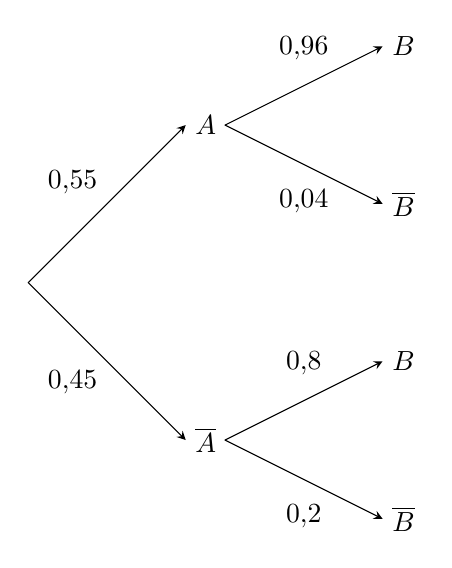
\begin{tikzpicture}[>=stealth,line cap=round,line join=round]
					\draw [->] (0,0)--(2,2) node [right]  {$A$};
					\draw[->] (0,0)--(2,-2)  node [right] {$\overline{A}$};
					\draw[->]  (2.5,2)--(4.5,3) node [right] {$B$};
					\draw[->] (2.5,2)--(4.5,1) node [right]  {$\overline{B}$};
					\draw[->] (2.5,-2)--(4.5,-1) node [right]  {$B$};
					\draw[->]  (2.5,-2)--(4.5,-3) node [right] {$\overline{B}$};
					 \path
						(0,0)--(2,2)  node [pos=.5,above left] {$0{,}55$}
						(0,0)--(2,-2) node  [pos=.5,below left] {$0{,}45$}
						 (2.5,2.2)--(4.5,3.2) node [pos=.5,above] {$0{,}96$}
						(2.5,1.8)--(4.5,0.8) node  [pos=.5,below] {$0{,}04$}
						(2.5,-1.8)--(4.5,-0.8)  node [pos=.5,above] {$0{,}8$}
						(2.5,-2.2)--(4.5,-3.2)  node [pos=.5,below] {$0{,}2$};
				\end{tikzpicture}
		\end{center}
		$\mathrm{P}(\overline{A}|B)=\dfrac{P(\overline{A})\mathrm{P}(B|\overline{A})}{\mathrm{P}(B)}=\dfrac{0{,}45\cdot0{,}8}{0{,}55\cdot0{,}96+0{,}45\cdot0{,}8}\approx 0{,}41$. 
	 }
\end{ex}

% nguồn: Lop_12_Dai_so_Chuong_6
\begin{ex}%[2D6V2-4]%[ma:37245997]
	Người ta điều tra thấy ở một địa phương nọ có $3\%$ tài xế sử dụng điện thoại di động khi lái xe. Người ta nhận thấy khi tài xế lái xe gây  ra tai nạn thì có $21\%$ là do tài xế sử dụng điện thoại. Hỏi việc sử dụng điện thoại di động khi lái xe làm tăng xác suất gây tai nạn lên bao nhiêu lần?
	\choice 
		 {$3$}
		{\True $7$} 
		{$5$} 
		 {$6$}
	 \loigiai{
		Ta gọi $A$ là biến cố \lq\lq Tài xế sử dụng điện thoại di động  khi lái xe\rq\rq , $B$ là biến cố \lq\lq Tài xế lái xe gây tai nạn\rq\rq .\\
		Khi đó  $\mathrm{P}\left(A\right)=3\%=0{,}03$; $\mathrm{P} \left(A|B\right)=21\%=0{,}21$.\\
		Theo  công thức Bayes ta có
		\[\mathrm{P}  \left(B|A\right)=\dfrac{\mathrm{P} \left(B\right)\mathrm{P} \left(A|B\right)}{\mathrm{P}\left(A\right)} \Rightarrow \dfrac{\mathrm{P} \left(B|A\right)}{\mathrm{P}\left(B\right)} =\dfrac{\mathrm{P} \left(A|B\right)}{P\left(A\right)}=\dfrac{0{,}21}{0{,}03}=7.\]
	Vậy việc sử dụng điện thoại di  động khi lái xe làm tăng xác suất gây tai nạn lên $7$ lần.}
\end{ex}


%%%%%%%%%%%%%%%% ĐÚNG/SAI %%%%%%%%%%%%%%%%

% nguồn: Lop_12_Dai_so_Chuong_6
\begin{ex}%[2D6H2-4]%[ma:e7d78428]
	Một kho hàng có $1\,000$ thùng hàng với bề ngoài giống hệt nhau, trong đó có $480$ thùng  hàng loại I và $520$ thùng hàng loại II. Trong số các thùng hàng đó, có $80\% $ thùng hàng loại I và $85\% $ thùng hàng loại II đã được kiểm định. Chọn ngẫu nhiên một thùng hàng trong kho.
	\choiceTF 
		{\True Xác  suất chọn được thùng hàng loại I bằng $48\% $}
		{Xác suất chọn được thùng hàng loại II đã được kiểm định bằng  $38{,}4\%$}
		 {\True Xác suất chọn được thùng hàng chưa kiểm định bằng $17{,}4\%$}
		{Giả sử thùng  hàng được lấy ra là thùng hàng chưa được kiểm định, xác suất thùng hàng đó là thùng loại I thấp hơn xác suất thùng hàng đó là thùng loại II}
	 \loigiai{
		Xét phép thử  chọn ngẫu nhiên một thùng hàng trong kho.\\
		Gọi $A$  là biến cố \lq\lq Chọn được thùng hàng loại I\rq\rq.\\
		$B$ là biến cố \lq\lq Chọn được thùng hàng đã  được kiểm định\rq\rq.\\
		Theo bài ra ta  có $\mathrm{P}\left(B\mid A\right)=80\%$, $\mathrm{P}\left(B\mid\overline A\right)=85\% $.
		\begin{itemchoice}
			\itemch Xác suất  chọn được thùng hàng loại I là $\mathrm{P}(A)=\dfrac{480}{1000}=48\% $.
			\itemch Ta có $\mathrm{P}\left(\overline  A\right)=\dfrac{520}{1000}=52\% $, $\mathrm{P}\left(B\mid\overline A\right)=85\% $.\\
			Xác suất chọn được thùng  hàng loại II đã được kiểm định là
			\[\mathrm{P}\left(\overline A\cap B\right)=\mathrm{P}\left(\overline A\right)\cdot\mathrm{P}\left(B\mid\overline A\right)=52\% \cdot85\%=44{,}2\%  .\]
			\itemch Xác suất chọn được thùng hàng  đã được kiểm định là
			\[\mathrm{P}(B)=\mathrm{P}(A)\cdot\mathrm{P}\left(B\mid A\right)+\mathrm{P}\left(\overline A\right)\cdot\mathrm{P}\left(B\mid\overline A\right)=48\%  \cdot80\%+52\% \cdot85\%=82{,}6\%.\]
			Suy  ra xác suất chọn được thùng hàng chưa kiểm định là $\mathrm{P}\left(\overline B\right)=1-\mathrm{P}(B)=17{,}4\% $.
			\itemch Giả sử thùng hàng được lấy ra  là thùng hàng chưa được kiểm định.\\
			Xác suất thùng hàng đó là thùng loại I là $$\mathrm{P}\left(A\mid\overline  B\right)=\dfrac{\mathrm{P}(A)\cdot\mathrm{P}\left(\overline B\mid A\right)}{\mathrm{P}\left(\overline B\right)}=\dfrac{48\% \cdot\left(1-80\%\right)}{17{,}4\%}=\dfrac{16}{29}.$$
			Xác suất thùng hàng đó là  thùng loại II là $$\mathrm{P}\left(\overline A\mid\overline B\right)=\dfrac{\mathrm{P}\left(\overline A\right)\cdot\mathrm{P}\left(\overline B\mid A\right)}{\mathrm{P}\left(\overline B\right)}=\dfrac{52\% \cdot\left(1-85\%\right)}{17{,}4\%}=\dfrac{13}{29}.$$
			Vây xác suất thùng hàng đó là thùng loại I cao hơn xác suất thùng hàng đó là thùng loại  II.
		\end{itemchoice}
	 }
\end{ex}

% nguồn: Lop_12_Dai_so_Chuong_6
\begin{ex}%[2D6H2-4]%[ma:0c891e39]
	Một hộp có $80$ viên bi, trong đó có $50$ viên bi màu đỏ và $30$ viên bi màu vàng; các viên bi có kích thước và khối lượng như nhau. Sau khi kiểm tra, người ta thấy có $60\%$ số viên  bi màu đỏ đánh số và $50\%$ số viên bi màu vàng có đánh số, những viên bi còn lại không đánh số. Lấy ra ngẫu nhiên 1 viên bi trong hộp.
	\choiceTF 
		 {\True Xác suất chọn được viên bi màu đỏ bằng $62{,}5\% $}
		{Xác suất chọn được viên bi màu vàng có đánh số  bằng $18{,}57\%$}
		{\True Xác suất  chọn được viên bi không đánh số bằng $43{,}75\%$}
		{Giả sử viên bi được lấy ra là viên bi chưa được đánh số, xác suất để viên bi đó là bi đỏ thấp hơn xác suất viên bi  đó là bi vàng}
	\loigiai{ 
		Xét phép thử chọn ngẫu nhiên  một viên bi.\\
		Gọi $A$ là biến cố \lq\lq Chọn được viên bi màu đỏ\rq\rq; $B$ là biến cố \lq\lq Chọn được viên bi đã được đánh số\rq\rq. Theo bài ra  ta có $\mathrm{P}\left(B\mid A\right)=60\%$, $\mathrm{P}\left(B\mid\overline A\right)=50\%$.
		\begin{itemchoice}
			\itemch Xác suất chọn được viên bi màu đỏ là $\mathrm{P}(A)=\dfrac{50}{80}=62{,}5\%$. 
			\itemch Ta có $\mathrm{P}\left(\overline A\right)=\dfrac{30}{80}=37{,}5\%  $, $\mathrm{P}\left(B\mid\overline A\right)=50\% $.\\
			Xác  suất chọn được viên bi màu vàng đã được đánh số là
			 \[\mathrm{P}\left(\overline A\cap B\right)=\mathrm{P}\left(\overline A\right)\cdot\mathrm{P}\left(B\mid\overline A\right)=37{,}5\% \cdot50\%=18{,}75\%.\]
			\itemch Xác suất chọn  được viên bi đã được đánh số là
			\[\mathrm{P}(B)=\mathrm{P}(A)\cdot\mathrm{P}\left(B\mid A\right)+\mathrm{P}\left(\overline A\right)\cdot\mathrm{P}\left(B\mid\overline A\right)=62{,}5\% \cdot60\%+37{,}5\% \cdot50\%=56{,}25\%.\] 
			Suy ra xác suất chọn được viên  bi chưa đánh số là $\mathrm{P}\left(\overline B\right)=1-\mathrm{P}(B)=43{,}75\% $.
			\itemch Giả sử viên bi được lấy ra là  viên bi chưa được đánh số. Khi đó\\
			Xác suất để viên bi đó là bi đỏ là $$\mathrm{P}\left(A\mid\overline B\right)=\dfrac{\mathrm{P}(A)\cdot\mathrm{P}\left(\overline B\mid A\right)}{\mathrm{P}\left(\overline B\right)}=\dfrac{62{,}5\% \cdot\left(1-60\%\right)}{43{,}75\%}=\dfrac{4}{7}.$$ 
			Xác suất để viên bi đó  là bi vàng là
			$$\mathrm{P}\left(\overline A\mid  \overline B\right)=1-\mathrm{P}\left(A\mid \overline{B}\right)=\dfrac{3}{7}.$$
			Vây xác suất viên bi đó là bi đỏ cao hơn xác  suất viên bi đó là bi xanh.
		\end{itemchoice}
	} 
\end{ex}

% nguồn: Lop_12_Dai_so_Chuong_6
\begin{ex}%[2D6H2-4]%[ma:31d0fbc8]
	Một cửa hàng có  hai máy sản xuất bánh ngọt. Máy thứ nhất sản xuất $70\%$ tổng số bánh của cửa hàng. Tỉ lệ bánh bị cháy của máy thứ nhất và máy thứ hai lần lượt là $5\%$ và $8\%$. Lấy ngẫu nhiên một chiếc bánh trong lô hàng của cửa hàng. Gọi $A$ là biến cố \lq\lq Chiếc bánh được sản xuất từ nhà máy thứ nhất\rq\rq\, và $B$ là biến cố \lq\lq Chiếc bánh bị cháy\rq\rq.
	\choiceTF 
		{\True  $\mathrm{P}(A)=0{,}7$ và $\mathrm{P}\left(\overline{A}\right)=0{,}3$}
		{\True Xác suất để lấy được bánh  bị cháy là $0{,}059$}
		{\True Nếu đã lấy được bánh bị cháy, xác suất bánh đó do máy thứ nhất  sản xuất là $0{,}59$ (kết quả được làm tròn đến hàng phầm trăm)}
		{Nếu lấy được bánh không bị cháy, tỉ lệ bánh  đó do máy hai sản xuất là $30\%$ (kết quả tính theo phần trăm được làm tròn đến hàng đơn vị)}
	 \loigiai{
		\begin{itemchoice}
			\itemch Ta  có $\mathrm{P}(A)=0{,}7$ và $\mathrm{P}\left(\overline{A}\right)=0{,}3$.
			 \itemch Xác suất lấy được bánh bị cháy là $$\mathrm{P}(B)=\mathrm{P}(A)\cdot \mathrm{P}(B\mid A)+\mathrm{P}\left(\overline{A}\right)\cdot \mathrm{P}\left(B\mid\overline{A}\right)=0{,}7\cdot{,}05+0{,}3\cdot 0{,}08=0{,}059.$$
			\itemch Ta có  $\mathrm{P}(A\mid B)=\dfrac{\mathrm{P}(A)\cdot\mathrm{P}(B|A)}{\mathrm{P}(B)}=\dfrac{0{,}7\cdot0{,}05}{0{,}059}\approx 0{,}59$.
			\itemch Ta có $\mathrm{P}\left(\overline{A}\mid \overline{B}\right)=\dfrac{\mathrm{P}\left(\overline{A}\right)\cdot\mathrm{P}\left(\overline{B}\mid \overline{A}\right)}{\mathrm{P}\left(\overline{B}\right)}=\dfrac{0{,}3\cdot0{,}08}{1-0{,}059}\approx  0{,}03$ hay $3\%$.
		\end{itemchoice}
	} 
\end{ex}

% nguồn: Lop_12_Dai_so_Chuong_6
\begin{ex}%[2D6H2-4]%[ma:1c5f1de4]
	Có hai đội tham gia một cuộc thi bơi lội. Đội I có $7$ vận động viên, đội II có  $9$ vận động viên. Xác suất giành huy chương vàng của mỗi vận động viên đội I và đội II lần lượt là $0{,}07$ và $0{,}06$. Chọn ngẫu nhiên một vận động viên.
	 \choiceTF
		{Xác suất để vận động viên  được chọn thuộc đội I là $\dfrac{9}{16}$}
		{\True Xác suất để vận động viên này không giành được huy chương vàng nếu thuộc đội II  là $0{,}94$}
		{Xác suất để vận động viên này giành được huy chương  vàng là $\dfrac{103}{1\,060}$}
		{\True Giả sử vận động viên được chọn giành huy chương vàng. Xác suất để vận động  viên này thuộc đội I là $\dfrac{49}{103}$}
	\loigiai{ 
		\begin{itemchoice}
			\itemch Xác  suất để vận động viên chọn ra thuộc đội I là $\dfrac{7}{16}$.
			\itemch Xác suất  không đạt huy chương vàng của mỗi vận động viên đội II là $1-0{,}06=0{,}94$.
			\itemch Gọi $A$ là biến cố \lq\lq Vận động viên đạt huy chương vàng\rq\rq, $B$ là biến cố \lq\lq Thành viên đội I\rq\rq thì biến cố đối của $B$ là $\overline B\colon $ \lq\lq Thành viên  đội II\rq\rq.\\
			Do đó, $\mathrm{P}(B)=\dfrac{7}{16};\,\mathrm{P}\left(\overline B\right)=\dfrac{9}{16}$; $\mathrm{P}\left(A\mid  B\right)=0{,}07$; $\mathrm{P}\left(A\mid\overline B\right)=0{,}06$.\\
			 Theo công thức xác suất toàn phần ta có
			\[\mathrm{P}(A)=\mathrm{P}(B)\cdot\mathrm{P}\left(A\mid  B\right)+\mathrm{P}\left(\overline B\right)\cdot\mathrm{P}\left(A\mid\overline B\right)=\dfrac{7}{16}\cdot0{,}07+\dfrac{9}{16}\cdot0{,}06=\dfrac{103}{1\,600}.\]
			\itemch Ta có $\mathrm{P}\left(B\mid A\right)=\dfrac{\mathrm{P}(B)\cdot \mathrm{P}\left(A\mid B\right)}{\mathrm{P}(A)}=\dfrac{\dfrac{7}{16}\cdot 0{,}07}{\dfrac{103}{1\,600}}=\dfrac{49}{103}$. 
		\end{itemchoice}
	 }
\end{ex}

% nguồn: Lop_12_Dai_so_Chuong_6
\begin{ex}%[2D6V2-4]%[ma:b6728b44]
	Một nhà máy có hai phân xưởng $X$ và $Y$ cùng sản xuất một loại sản phẩm. Phân xưởng $X$ sản xuất $60\% $ và phân xưởng $Y$ sản xuất $40\% $ tổng số sản phẩm của cả nhà máy.  Tỉ lệ phế phẩm của phân xưởng $X$, phân xưởng $Y$ lần lượt là $10\%$ và $5\%$. Lấy ngẫu nhiên một sản phẩm trong kho hàng của nhà máy.
	\choiceTF 
		{Xác suất lấy được sản phẩm phẩm tốt, biết sản phẩm đó do  phân xưởng $X$ sản xuất bằng $95\%$}
		{Xác suất lấy được  phế phẩm là $10\%$}
		{\True Giả sử đã lấy được phế phẩm, xác suất  phế phẩm đó do phân xưởng $Y$ sản xuất bằng $75\%$}
		{\True Nếu lấy được sản phẩm tốt, khả năng sản phẩm đó do phân xưởng $X$  sản xuất cao hơn khả năng sản phẩm đó do phân xưởng $Y$ sản xuất}
	 \loigiai{
		Xét phép thử lấy ngẫu nhiên một  sản phẩm trong kho hàng của nhà máy.\\
		Gọi $A$  là biến cố \lq\lq Lấy được sản phẩm do phân xưởng $X$ sản xuất\rq\rq.\\
		$\overline A$ là biến cố \lq\lq Lấy  được sản phẩm do phân xưởng $Y$ sản xuất\rq\rq.\\
		$B$  là biến cố \lq\lq Lấy được phế phẩm\rq\rq.\\
		$\overline B$ là biến cố  \lq\lq Lấy được sản phẩm tốt\rq\rq.\\
		Theo  bài ra ta có $\mathrm{P}(A)=60\%$, $\mathrm{P}(A)=40\% $, $\mathrm{P}\left(B\mid A\right)=10\% $, $\mathrm{P}\left(B\mid\overline A\right)=5\% $.
		\begin{itemchoice}
			 \itemch Xác suất lấy được sản phẩm phẩm tốt, biết sản phẩm đó do phân xưởng $X$ sản xuất là xác suất có điều kiện $\mathrm{P}\left(\overline B\mid A\right)=1-\mathrm{P}\left(B\mid A\right)=90\% $.
			\itemch Xác suất lấy  được phế phẩm là
			\[\mathrm{P}(B)=\mathrm{P}(A)\cdot\mathrm{P}\left(B\mid A\right)+\mathrm{P}\left(\overline A\right)\cdot\mathrm{P}\left(B\mid\overline  A\right)=60\% \cdot10\%+40\% \cdot5\%=8\%.\]
			\itemch Giả sử đã lấy  được phế phẩm, xác suất phế phẩm đó do phân xưởng $Y$ sản xuất là xác suất có điều kiện $\mathrm{P}\left(A\mid B\right)$. Ta có $\mathrm{P}\left(A\mid B\right)=\dfrac{\mathrm{P}(A)\cdot\mathrm{P}\left(B\mid A\right)}{\mathrm{P}(B)}=\dfrac{60\% \cdot10\%}{8\%}=75\% $.
			\itemch Ta có $\mathrm{P}\left(\overline  B\right)=1-\mathrm{P}(B)=1-8\%=92\% $; $\mathrm{P}\left(\overline B\mid A\right)=90\% $;\\
			$\mathrm{P}\left(\overline B\mid\overline A\right)=1-\mathrm{P}\left(B\mid\overline  A\right)=1-5\%=95\% $.\\
			Nếu lấy được sản phẩm tốt thì xác suất sản  phẩm đó do phân xưởng $X$ sản xuất là $$\mathrm{P}\left(A\mid\overline B\right)=\dfrac{\mathrm{P}(A)\cdot \mathrm{P}\left(\overline B\mid A\right)}{\mathrm{P}\left(\overline B\right)}=\dfrac{60\% \cdot90\%}{92\%}=\dfrac{27}{46}.$$
			Xác suất sản phẩm đó do phân xưởng $Y$ sản xuất là $$\mathrm{P}\left(\overline A\mid\overline B\right)=\dfrac{\mathrm{P}\left(\overline  A\right)\cdot\mathrm{P}\left(\overline B\mid\overline A\right)}{\mathrm{P}\left(\overline B\right)}=\dfrac{40\% \cdot95\%}{92\%}=\dfrac{19}{46}.$$
			Vì $\dfrac{27}{46}>\dfrac{19}{46}$ nên nếu lấy được sản phẩm tốt, khả năng sản phẩm đó do phân xưởng $X$ sản xuất cao hơn  khả năng sản phẩm đó do phân xưởng $Y$ sản xuất.
		\end{itemchoice}
	} 
\end{ex}

% nguồn: Lop_12_Dai_so_Chuong_6
\begin{ex}%[2D6V2-4]%[ma:70222491]
	Trong kỳ kiểm tra  môn Toán của một trường THPT có $400$ học sinh tham gia, trong đó có $180$ học sinh nam và $220$ học sinh nữ. Khi công bố kết quả kỳ kiểm tra đó, tỉ lệ học sinh đạt điểm giỏi tương ứng với nam và nữ lần lượt là $25\%$ và $30\%$. Chọn ngẫu nhiên một học sinh trong số $400$ học sinh đó.\\
	Gọi $A$ là  biến cố \lq\lq Học sinh được chọn ra đạt điểm giỏi \rq\rq, $B$ là biến cố \lq\lq Học sinh được chọn ra là học sinh nữ \rq\rq.
	 \choiceTF
		{\True Xác suất  $\mathrm{P}(B)=\dfrac{9}{20}$ và $\mathrm{P}(\overline{B})=\dfrac{11}{20}$}
		{Xác suất có  điều kiện $\mathrm{P}(A \mid \overline{B})=0{,}3$}
		{\True Xác  suất $\mathrm{P}(\overline{A})=0{,}7225$}
		{\True Trong số học  sinh đạt điểm giỏi có $59\%$ học sinh nữ đạt điểm giỏi trong kì kiểm tra môn Toán (kết quả làm tròn đến hàng đơn vị)}
	 \loigiai{
		\begin{itemchoice}
			\itemch Ta có $\mathrm{P}(B) = \dfrac{220}{400}=\dfrac{11}{20}$  và $\mathrm{P}\left(\overline{B}\right) =\dfrac{180}{440}= \dfrac{9}{20}$.
			\itemch Xác suất có điều kiện $\mathrm{P}(A  \mid \overline{B})$ là $\mathrm{P}\left(A\mid \overline{B}\right)=0{,}25$.
			\itemch Áp dụng công  thức xác suất toàn phần, ta có
			\[\mathrm{P}(A)= \mathrm{P}(B) \cdot \mathrm{P}\left(A  \mid B\right)+\mathrm{P}\left(\overline{B}\right) \cdot \mathrm{P}\left(A \mid \overline{B}\right)= \dfrac{11}{20} \cdot 0{,}3+\dfrac{9}{20} \cdot 0{,}25=0{,}2775.\]
			 Khi đó
			\[\mathrm{P}\left(\overline{A}\right)=1-\mathrm{P}(A)=1-0{,}2775=0{,}7225.\] 
			\itemch Trong  số học sinh đạt điểm giỏi, xác suất để bạn đó là học sinh nữ là
			\[\mathrm{P}(B \mid A) =\dfrac{\mathrm{P}(B) \cdot \mathrm{P}(A \mid B)}{\mathrm{P}(A)}=\dfrac{\dfrac{11}{20} \cdot 0{,}3}{0{,}2775}=\dfrac{22}{37}  \approx 59\%.\]
		\end{itemchoice}
	} 
\end{ex}

% nguồn: Lop_12_Dai_so_Chuong_6
\begin{ex}%[2D6V2-4]%[ma:72acde37]
	Một kho hàng có $1\,000$ thùng hàng với bề ngoài giống hệt nhau, trong đó có $480$ thùng hàng loại $I$ và $520$ thùng hàng loại $II$. Trong số các thùng hàng đó, có $80\%$ thùng hàng loại $I$ và $85\%$ thùng hàng loại $II$ đã được kiểm định. Chọn ngẫu nhiên một thùng hàng trong kho. Xét tính đúng sai của  các khẳng định sau
	 \choiceTF
		{\True Xác suất chọn được thùng  hàng loại $I$ bằng $48\%$}
		{Xác suất chọn được thùng hàng loại $II$ đã được kiểm  định bằng $38{,}4\%$}
		{\True Xác suất  chọn được thùng hàng chưa kiểm định bằng $17{,}4\%$}
		{Giả sử thùng hàng được lấy ra là thùng hàng chưa được kiểm định, xác suất thùng hàng đó là thùng loại $I$  thấp hơn xác suất thùng hàng đó là thùng loại $II$}
	 \loigiai{
		 Gọi
		\begin{itemize}
			\item $A$ là biến cố chọn được  thùng hàng loại $I$.
			\item $\overline{A}$ là biến cố chọn được thùng  hàng loại $II$.
			\item $C$ là biến cố  chọn được thùng hàng đã được kiểm định.
			\item $\overline{C}$ là biến cố  chọn được thùng hàng chưa được kiểm định.
		\end{itemize}
		\begin{center}
			\begin{tikzpicture}[scale=.5,font=\footnotesize,line join=round,line cap=round,>=stealth]
					 \coordinate (O) at (2,-1);
					\begin{scope}[ethicknode/.style={circle,draw,fill=red!10}]
						\node (D2) at (9,3) {$A$}; 
						\node (D3)  at (9,-5) {$\overline{A}$};
						\node  (B3) at (16,5) {$C$};
						\node (B4) at (16,1) {$\overline{C}$}; 
						\node (B5) at  (16,-3) {$C$};
						\node  (B6) at (16,-7) {$\overline{C}$};
					\end{scope}
					 \node[right=0.8cm of B3] {Đã được kiểm định};
					\node[right=0.8cm  of B4] {Chưa được kiểm định};
					\node[right=0.8cm of B5] {Đã  được kiểm định};
					\node[right=0.8cm  of B6] {Chưa được kiểm định};
					 \draw[->] (O)--(D2) node[midway,above] {$0{,}48$};
					 \draw[->] (O)--(D3) node[midway,below] {$0{,}52$};
					\draw[->]  (D2)--(B3) node[midway,above] {$0{,}8$};
					\draw[->] (D2)--(B4) node[midway,below]  {$0{,}2$};
					 \draw[->] (D3)--(B5) node[midway,above] {$0{,}85$};
					\draw[->] (D3)--(B6)  node[midway,below] {$0{,}15$};
				\end{tikzpicture}
		\end{center}
		Theo đề bài, ta  có
		\begin{itemize}
			\item  $P(A)=\dfrac{480}{1000}=0{,}48$.
			\item $P(\overline{A})=\dfrac{520}{1000}=0{,}52$. 
			\item  $P(C\mid A)=80\%=0{,}8$.
			 \item $P(C\mid \overline{A})=85\%=0{,}85$.
			\item  $P(\overline{C}\mid A)=1-0{,}8=0{,}2$.
			\item  $P(\overline{C}\mid \overline{A})=1-0{,}85=0{,}15$.
		\end{itemize}
		\begin{itemchoice}
			\itemch \textbf{Đúng}. Xác suất chọn được thùng hàng loại $I$ là  $P(A)=\dfrac{480}{1000}=0{,}48$.
			\itemch \textbf{Sai}. Xác suất chọn được thùng hàng loại $II$  đã được kiểm định là
			\begin{eqnarray*}
				P(\overline{A}\cap C)=P(C\mid  \overline{A})\cdot P(\overline{A})=0{,}85\cdot0{,}52=0{,}442.
			\end{eqnarray*}
			\itemch \textbf{Đúng}. Áp dụng công thức xác suất toàn phần, xác  suất để chọn được thùng hàng chưa được kiểm định là
			\begin{align*}
				P(\overline{C}) &= P(\overline{C}\mid A) \cdot P(A) +  P(\overline{C}\mid \overline{A}) \cdot P(\overline{A}) \\
				 &= 0{,}2 \cdot 0{,}48 + 0{,}15 \cdot 0{,}52 \\
				 &= 0{,}096 + 0{,}078 \\
				 &= 0{,}174.
			\end{align*}
			\itemch \textbf{Sai}. Ta cần so sánh $P(A\mid\overline{C})$  và $P(\overline{A}\mid\overline{C})$.\\
			Sử dụng công thức Bayes ta có 
			\begin{eqnarray*}
				&&P(A\mid  \overline{C})=\dfrac{P(\overline{C}\mid A)\cdot P(A)}{P(\overline{C})}=\dfrac{0{,}2\cdot0{,}48}{0{,}174}=\dfrac{0{,}096}{0{,}174}.\\
				&&P(\overline{A}\mid \overline{C})=\dfrac{P(\overline{C}\mid  \overline{A})\cdot P(\overline{A})}{P(\overline{C})}=\dfrac{0{,}15\cdot0{,}52}{0{,}174}=\dfrac{0{,}078}{0{,}174}.
			\end{eqnarray*}
			Vì $0{,}096>0{,}078$  nên $P(A\mid\overline{C})>P(\overline{A}\mid\overline{C})$.
		\end{itemchoice}
	 }
\end{ex}


%%%%%%%%%%%%%%%% TRẢ LỜI NGẮN %%%%%%%%%%%%%%%%

% nguồn: Lop_12_Dai_so_Chuong_6
\begin{bt}%[2D6H2-4]%[ma:275eb150]
	Một cặp sinh đôi có thể sinh đôi cùng trứng hoặc sinh đôi khác trứng. Các cặp sinh đôi cùng trứng luôn cùng giới tính. Đối với cặp sinh đôi khác trứng, thì giới tính của mỗi đứa trẻ là độc lập và có xác suất $0{,}5$ là con trai. Một thống kê cho thấy, có khoảng $34\%$ cặp sinh đôi đều là trai, $30\%$ cặp sinh đôi đều là gái, $36\%$ cặp sinh đôi là một trai và một gái. Chọn ngẫu nhiên một cặp sinh đôi. Tính xác suất để cặp sinh đôi đó là sinh đôi cùng trứng, biết cặp sinh đôi đó cùng giới tính (làm tròn kết quả đến hàng phần trăm). 
	\shortans{0,44} 
	\loigiai{ 
		 Gọi
		\begin{itemize}
			\item $A$ là biến cố \lq\lq cặp sinh đôi đó là sinh đôi cùng  trứng\rq\rq.
			\item $B$ là biến cố \lq\lq cặp sinh đôi đó cùng giới  tính\rq\rq.
		\end{itemize}
	 }
	Từ giả thiết của đề bài ta có $P(B \mid A)=1$, $P(B \mid  \overline{A})=0{,}5$ và $P(B)=0{,}3+0{,}34=0{,}64$.\\
	Áp dụng công thức xác suất toàn phần, ta  có
	\[P(B)=P(A) \cdot P(B \mid A) +P(\overline{A}) \cdot P(\overline{A})=P(A) \cdot 1 +\left[1-P(A)\right]  \cdot P(B\mid \overline{A})=0{,}64 \Leftrightarrow P(A)=0{,}28.\]
	 Áp dụng công thức Bayes, ta có
	\[P(A \mid B) =\dfrac{P(A) \cdot P(B \mid A)}{P(B)}=\dfrac{0{,}28 \cdot 1}{0{,}64}  \approx 0{,}44.\]
\end{bt}

% nguồn: Lop_12_Dai_so_Chuong_6
\begin{bt}%[2D6H2-4]%[ma:e9fb9ace]
	Trong một lễ hội mùa hè, có một trò chơi mà mỗi lần chơi, người chơi sẽ tung đồng thời bốn đồng xu cân đối một cách ngẫu nhiên. Người chơi chỉ thắng cuộc nếu nhận được ít nhất ba mặt ngửa từ bốn đồng xu đã tung. Tính xác suất để trong  $5$ lần chơi, người chơi thắng được ít nhất ba lần? (làm tròn kết quả đến hàng phần trăm).
	 \shortans{0,02}
	 \loigiai{
		\textbf{Bước 1:} Tính xác suất thắng trong một lần  chơi.\\
		Trong một lần chơi, người  chơi tung $4$ đồng xu cân đối
		\begin{itemize}
			\item Xác suất nhận được đúng $3$ mặt ngửa là $\mathrm{C}_4^3\cdot \left(\dfrac{1}{2}\right)^3\cdot \left(\dfrac{1}{2}\right)^1 = 4\cdot \dfrac{1}{8}\cdot  \dfrac{1}{2} = 4\cdot \dfrac{1}{16} = \dfrac{1}{4}$.
			\item Xác suất  nhận được cả $4$ mặt ngửa là $\left(\dfrac{1}{2}\right)^4 = \dfrac{1}{16}$.
		\end{itemize}
		Vậy xác suất thắng trong một lần chơi là $\dfrac{1}{4} +  \dfrac{1}{16} = \dfrac{5}{16}$.\\
		Xác suất thua trong một  lần chơi là $1 - \dfrac{5}{16} = \dfrac{11}{16}$.\\
		\textbf{Bước 2:} Tính xác  suất thắng ít nhất $3$ lần trong $5$ lần chơi.\\
		 Xác suất này bao gồm các trường hợp:
		\begin{itemize}
			\item Thắng đúng $3$ lần, thua $2$ lần $\mathrm{C}_5^3\cdot \left(\dfrac{5}{16}\right)^3\cdot \left(\dfrac{11}{16}\right)^2 = 10\cdot \dfrac{125}{4096}\cdot  \dfrac{121}{256} = \dfrac{151\,250}{1\,048\,576}$.
			\item Thắng đúng $4$ lần, thua $1$ lần $\mathrm{C}_5^4\cdot  \left(\dfrac{5}{16}\right)^4\cdot \left(\dfrac{11}{16}\right)^1 = 5\cdot \dfrac{625}{65\,536}\cdot \dfrac{11}{16} = \dfrac{34\,375}{1\,048\,576}$.
			\item  Thắng cả $5$ lần: $\left(\dfrac{5}{16}\right)^5 = \dfrac{3\,125}{1\,048\,576}$.
		\end{itemize}
		Xác suất cần tính là \[\dfrac{151\,250}{1\,048\,576} + \dfrac{34\,375}{1\,048\,576}  + \dfrac{3\,125}{1\,048\,576} \approx 0{,}02.\]
	} 
\end{bt}

% nguồn: Lop_12_Dai_so_Chuong_6
\begin{bt}%[2D6H2-4]%[ma:6e84cc19]
	Tại một địa phương có $500$ người cao tuổi, bao gồm $260$ nam và $240$ nữ. Trong đó nhóm người cao tuổi nam và nữ lần lượt có $40\%$ và $55\%$ bị bệnh tiểu đường. Chọn  ngẫu nhiên một người. Xác suất để chọn được một người không bị bệnh tiểu đường là bao nhiêu (làm tròn kết quả đến chữ số hàng phần trăm)?
	\shortans{0,53} 
	\loigiai{ 
		 Xét các biến cố:\\
		$A\colon$ \lq\lq  Chọn được người không bị tiểu đường\rq\rq.\\
		$B\colon$ \lq\lq Chọn  được người cao tuổi là nam\rq\rq.\\
		$\overline B$ \lq\lq Chọn được  người cao tuổi là nữ\rq\rq.\\
		Từ  giải thuyết ta có $\mathrm{P}(B)=\dfrac{260}{500}=0{,}52$; $\mathrm{P}\left(A\mid B\right)=1-0{,}4=0{,}6$;\\
		$\mathrm{P}\left(\overline  B\right)=\dfrac{240}{500}=0{,}48$; $\mathrm{P}\left(A\mid\overline B\right)=1-0{,}55=0{,}45$.\\
		Theo công thức xác suất toàn phần, ta có 
		\[\mathrm{P}(A)=\mathrm{P}(B)\cdot\mathrm{P}\left(A\mid  B\right)+\mathrm{P}\left(\overline B\right)\cdot \mathrm{P}\left(A\mid\overline B\right)=0{,}52\cdot0{,}6+0{,}48\cdot0{,}45=0{,}528\approx 0{,}53.\]
	 }
\end{bt}

% nguồn: Lop_12_Dai_so_Chuong_6
\begin{bt}%[2D6V2-4]%[ma:e223811a]
	Một xét nghiệm Covid – 19 cho kết quả dương tính với $90\% $ các trường hợp thực sự nhiễm virus và cho  kết quả âm tính với $80\% $ các trường hợp thực sự không nhiễm virus. Biết rằng tỉ lệ người nhiễm Covid – 19 trong một cộng đồng nào đó là $1\% $. Một người trong cộng đồng đó cho kết quả xét nghiệm dương tính. Xác suất để người đó thực sự bị nhiễm virus có dạng $\dfrac{a}{b}$ (phân số tối giản). Giá trị của $a+b$ bằng bao nhiêu?
	 \shortans{24}
	\loigiai{ 
		Gọi $A$ là biến cố \lq\lq Người đó bị nhiễm  Virus\rq\rq; $B$ là biến cố \lq\lq Người đó cho kết quả dương tính\rq\rq.\\
		Xét nghiệm Covid – 19 cho kết quả dương tính với $90\% $ các trường hợp  thực sự nhiễm virus $\mathrm{P}\left(B\mid A\right)=0{,}9$.\\
		Xét nghiệm Covid – 19 cho kết quả âm tính  với $80\% $ các trường hợp thực sự không nhiễm virus, nên cho kết quả dương tính với $20\% $ các trường hợp không thực sự nhiễm virus $\mathrm{P}\left(B\mid \overline A\right)=0{,}2$.\\
		$\mathrm{P}(A)=0{,}01\Rightarrow \mathrm{P}\left(\overline  A\right)=0{,}99$.\\
		Do đó xác suất để người đó cho  kết quả dương tính là
		\[\mathrm{P}(B)=\mathrm{P}(A)\cdot\mathrm{P}\left(B\mid  A\right)+\mathrm{P}\left(\overline A\right)\cdot\mathrm{P}\left(B\mid \overline A\right)=0{,}01\cdot0{,}9+0{,}99\cdot0{,}2=0{,}207.\]
		Xác suất để người  nhiễm virus cho kết quả dương tính là
		 \[\mathrm{P}\left(A\mid B\right)=\dfrac{\mathrm{P}(A)\cdot\mathrm{P}\left(B\mid A\right)}{\mathrm{P}(B)}=\dfrac{0{,}01\cdot0{,}9}{0{,}207}=\dfrac{1}{23}.\]
	Vậy  $a=1$, $b=23\Rightarrow a+b=24$.}
\end{bt}

% nguồn: Lop_12_Dai_so_Chuong_6
\begin{bt}%[2D6V2-4]%[ma:85ac542c]
	Có hai hộp. Hộp $I$ có $7$ quả cầu mầu xanh và còn lại là quả cầu mầu vàng. Hộp $II$ có $8$ quả cầu mầu xanh và $5$ quả cầu mầu vàng. Trước tiên lấy ra ngẫu nhiên một quả cầu từ hộp $I$ rồi thả vào hộp $II$. Sau đó lại lấy ra ngẫu nhiên $1$ quả cầu từ hộp $II$.  Xác suất để quả cầu lấy ra là quả cầu màu vàng là $\dfrac{95}{238}$. Tính số quả cầu mầu vàng có trong hộp $I$.
	\shortans{10} 
	 \loigiai{
		Gọi $x$ là số quả cầu mầu vàng có  trong hộp $I\,(x\in\mathbb{N})$. \\
		Hộp $I$ có $7$ xanh và  $x$ hay hộp $I$ có tổng cộng $7+x$ (viên bi). \\
		Gọi biến cố $A\colon$ \lq\lq Lấy được một quả cầu mầu xanh từ  hộp $I$\rq\rq. \\
		Suy ra $\overline{A}\colon$ \lq\lq Lấy được một  quả cầu mầu vàng từ hộp $I$\rq\rq. \\
		Và $B$ là biến cố \lq\lq Lấy được một  quả cầu mầu vàng từ hộp $II$\rq\rq. \\
		 Ta có $\mathrm{P}\left(A\right)=\dfrac{7}{7+x}$; $\mathrm{P}\left(\overline{A}\right)=\dfrac{x}{7+x}$. \\
		Nếu $A$ xảy ra (thêm $1$ xanh  vào $II$), khi đó hộp $II$ có $9$ xanh, $5$ vàng hay hộp $II$ có tổng cộng $14$ viên bi. Suy ra $\mathrm{P}\left(B\mid A\right)=\dfrac{5}{14}$. \\
		Nếu $\overline{A}$ xảy ra (thêm $1$ vàng vào $II$), hộp $II$ có $8$ xanh, $6$ vàng hay hộp $II$ có tổng cộng $14$ viên bi. Suy ra $\mathrm{P}\left(B\mid  \overline{A}\right)=\dfrac{6}{14}$. \\
		Áp dụng công thức xác suất toàn phần, ta được \\ $\mathrm{P}\left(B\right)=\mathrm{P}\left(A\right)\cdot\mathrm{P}\left(B\mid A\right)+\mathrm{P}\left(\overline{A}\right)\cdot\mathrm{P}\left(B\mid \overline{A}\right)=\dfrac{7}{7+x}\cdot\dfrac{5}{14}+\dfrac{x}{7+x}\cdot\dfrac{6}{14}=\dfrac{6x+35}{14(7+x)}$. \\ Theo đề bài 
		$$\mathrm{P}\left(B\right)=\dfrac{95}{238}\Leftrightarrow \dfrac{6x+35}{14(7+x)}=\dfrac{95}{238}\Leftrightarrow  102x+595=95x+665\Leftrightarrow x=10.$$
		Vậy số quả cầu mầu vàng trong hộp $I$ là  $10$.
	} 
\end{bt}

% nguồn: Lop_12_Dai_so_Chuong_6
\begin{bt}%[2D6V2-4]%[ma:cca43469]
	Một hộp chứa $10$ bi xanh và $5$ bi đỏ. Bạn An rút ngẫu nhiên $1$ bi, xem màu rồi bỏ ra ngoài. Nếu bi An rút được màu xanh thì bạn Bình sẽ rút $2$ bi; nếu bi An rút được màu đỏ thì bạn Bình sẽ rút $3$ bi (từ hộp còn lại). Biết rằng tất cả các viên bi được hai bạn chọn ra đều có đủ hai màu. Tính xác suất  An rút bi xanh.
	 \shortans{0,55}
	 \loigiai{
		Gọi $A$ là biến  cố \lq\lq An rút bi xanh\rq\rq\, và $B$ là biến cố \lq\lq tập bi được chọn có đủ hai màu\rq\rq.\\
		 Ta có
		 $\mathrm \mathrm{P}(A)=\dfrac{10}{15}=\dfrac{2}{3}$; $\mathrm{P}\left(\overline{A}\right)=\dfrac{1}{3}$.\\
		Nếu $A$ xảy ra khi đó hộp còn lại có $9$ bi xanh, $5$ bi đỏ. Khi đó, Bình rút $2$ bi có  ít nhất một bi đỏ
		\[ 
		\mathrm{P}(B\mid A)=1-\dfrac{\mathrm{C}_9^2}{\mathrm{C}_{14}^2}=\dfrac{55}{91}. 
		 \]
		Nếu  $\overline{A}$ xảy ra khi đó hộp còn lại có $10$ bi xanh, $4$ bi đỏ. Khi đó, Bình rút $3$ bi có ít nhất một xanh
		\[ 
		 \mathrm{P}(B\mid \overline{A})=1-\dfrac{\mathrm{C}_4^3}{\mathrm{C}_{14}^3}=\dfrac{90}{91}.
		 \]
		Theo công thức Bayes, ta  có
		 \[
		\mathrm{P}(A\mid  B)=\dfrac{\dfrac{2}{3}\cdot\dfrac{55}{91}}{\dfrac{2}{3}\cdot\dfrac{55}{91}+\dfrac{1}{3}\cdot\dfrac{90}{91}}=\dfrac{11}{20}=0{,}55.
		\] 
	} 
\end{bt}

% nguồn: Lop_12_Dai_so_Chuong_6
\begin{bt}%[2D6V2-4]%[ma:49b2306d]
	Trường THPT chuyên $X$ có bốn lớp chuyên bao gồm: Toán, Tin, Lý và Hóa. Theo thống kê, tỷ lệ học sinh lớp chuyên Toán trúng tuyển vào các ngành đại học top đầu là $65\%$, lớp chuyên Tin là $35\%$, lớp chuyên Lý là $55\%$ và chuyên Hóa là $45\%$. Biết rằng số học sinh lớp chuyên Toán gấp rưỡi số học sinh lớp chuyên Lý, số học sinh lớp chuyên Lý bằng số học sinh lớp chuyên Hóa, và số học sinh lớp chuyên Tin bằng $80\%$ số học sinh lớp chuyên Lý. Chọn ngẫu nhiên một học sinh của trường và biết rằng học sinh đó đã trúng tuyển vào các ngành đại học top đầu. Tính xác  suất để học sinh đó không phải là học sinh lớp chuyên Toán hoặc lớp chuyên Lý. (kết quả làm tròn đến hàng phần trăm).
	\shortans{0,32} 
	\loigiai{ 
		Gọi các biến cố  như sau
		\begin{itemize}
			\item $T$ là biến cố \lq\lq  Học sinh được chọn là học sinh lớp chuyên Toán\rq\rq;
			\item $I$ là biến cố \lq\lq Học sinh được chọn là học sinh lớp  chuyên Tin\rq\rq;
			\item $L$ là biến  cố \lq\lq Học sinh được chọn là học sinh lớp chuyên Lý\rq\rq;
			\item $H$ là biến cố \lq\lq Học sinh được chọn là học sinh lớp chuyên Hóa\rq\rq; 
			\item $X$ là biến cố \lq\lq Là  học sinh trúng tuyển vào các ngành đại học top đầu\rq\rq.
		\end{itemize}
		Khi đó $\mathrm{P}\left(X\mid T\right)=0{,}65$; $\mathrm{P}\left(X\mid I\right)=0{,}35$; $\mathrm{P}\left(X\mid L\right)=0{,}55$; $\mathrm{P}\left(X\mid H\right)=0{,}45$. \\ 
		Gọi số học sinh của lớp chuyên Lý là $x$ thì số học sinh lớp chuyên Tin, Hóa và Toán  lần lượt là $0{,}8x; x; 1{,}5x$ (học sinh). \\
		Tổng số học sinh  bốn lớp chuyên là $x+0{,}8x+x+1{,}5x=4{,}3x$. \\
		Khi đó $\mathrm{P}\left(T\right)=\dfrac{1{,}5x}{4{,}3x}=\dfrac{15}{43}$; $\mathrm{P}\left(I\right)=\dfrac{0{,}8x}{4{,}3x}=\dfrac{8}{43}$; $\mathrm{P}\left(L\right)=\dfrac{x}{4{,}3x}=\dfrac{10}{43}=\mathrm{P}\left(H\right)$.  \\
		Xác suất học sinh được trúng tuyển vào các ngành đại học top đầu là \\ $\mathrm{P}\left(X\right)=\mathrm{P}\left(X\mid T\right)\cdot\mathrm{P}\left(T\right)+\mathrm{P}\left(X\mid  I\right)\cdot\mathrm{P}\left(I\right)+\mathrm{P}\left(X\mid L\right)\cdot\mathrm{P}\left(L\right)+\mathrm{P}\left(X\mid H\right)\cdot\mathrm{P}\left(H\right)$. \\ $\mathrm{P}\left(X\right)=(0{,}65\cdot\dfrac{15}{43})+(0{,}35\cdot\dfrac{8}{43})+(0{,}55\cdot\dfrac{10}{43})+(0{,}45\cdot\dfrac{10}{43})=\dfrac{22{,}55}{43}=\dfrac{451}{860}$. \\
		Xác suất học sinh trúng tuyển vào các  ngành đại học top đầu từ lớp chuyên Hóa hoặc chuyên Tin là $$\mathrm{P}\left(X\cap(I\cup H)\right)=\mathrm{P}\left(X\mid H\right)\cdot\mathrm{P}\left(H\right)+\mathrm{P}\left(X\mid I\right)\cdot\mathrm{P}\left(I\right)=0{,}45\cdot\dfrac{10}{43}+0{,}35\cdot\dfrac{8}{43}=\dfrac{7{,}3}{43}=\dfrac{73}{430}.$$
		Vậy xác suất để học sinh này không phải là học sinh lớp chuyên  Toán hoặc lớp chuyên Lý là $$\mathrm{P}\left(I\cup H\mid X\right)=\dfrac{\mathrm{P}\left(X\cap(I\cup H)\right)}{\mathrm{P}\left(X\right)}=\dfrac{\dfrac{73}{430}}{\dfrac{451}{860}}=\dfrac{146}{451}\approx 0{,}32.$$
	} 
\end{bt}

% nguồn: Lop_12_Dai_so_Chuong_6
\begin{bt}%[2D6V2-4]%[ma:991cb994]
	Một nhà máy sản xuất linh kiện điện tử có ba dây chuyền sản xuất $A, B$ và $C$. Dây chuyền $A$ sản xuất $50\%$ số linh kiện, dây chuyền $B$ sản xuất $30\%$ và dây chuyền $C$ sản xuất $20\%$ số linh kiện. Tỷ lệ phế phẩm của từng dây chuyền lần lượt là $2\%, 3\%$ và $1\%$. Chọn một linh kiện ngẫu nhiên và phát hiện là phế phẩm thì xác suất để linh kiện đó được sản xuất từ dây chuyền $A$ là bao nhiêu? 
	 \shortans{0,48}
	 \loigiai{
		Gọi các  biến cố
		\begin{itemize}
			\item $A$: "Linh kiện được sản xuất  từ dây chuyền A".
			\item $B$: "Linh kiện được sản xuất từ dây chuyền  B".
			\item $C$: "Linh kiện được sản xuất từ  dây chuyền C".
			\item $D$: "Linh  kiện là phế phẩm".
		\end{itemize}
		Khi đó, ta  có
		\begin{multicols}{3}
			\begin{itemize}
				\item $\mathrm{P}\left(A\right)=0{,}5$; 
				\item  $\mathrm{P}\left(B\right)=0{,}3$;
				 \item $\mathrm{P}\left(C\right)=0{,}2$;
				\item  $\mathrm{P}\left(D\mid A\right)=0{,}02$;
				 \item $\mathrm{P}\left(D\mid B\right)=0{,}03$;
				 \item $\mathrm{P}(D\mid C)=0{,}01$.
			\end{itemize}
		\end{multicols}
		Xác suất để sản xuất một linh kiện phế phẩm là 
		\begin{align*}
			\mathrm{P}\left(D\right)&=\mathrm{P}\left(A\right)\cdot\mathrm{P}\left(D\mid A\right)+\mathrm{P}\left(B\right)\cdot\mathrm{P}\left(D\mid B\right)+\mathrm{P}\left(C\right)\cdot\mathrm{P}\left(D\mid  C\right)\\
			&=0{,}5\cdot0{,}02+0{,}3\cdot0{,}03+0{,}2\cdot0{,}01\\ 
			&=0{,}021. 
		\end{align*}
		Nếu chọn một linh kiện ngẫu nhiên và phát hiện là phế phẩm thì xác suất để linh kiện đó được sản xuất từ  dây chuyền $A$ là
		\[\mathrm{P}\left(A\mid D\right)=\dfrac{\mathrm{P}\left(A\right)\cdot\mathrm{P}\left(D\mid A\right)}{\mathrm{P}\left(D\right)}=\dfrac{0{,}5\cdot0{,}02}{0{,}021}=0{,}48.\] 
	} 
\end{bt}

% nguồn: Lop_12_Dai_so_Chuong_6
\begin{bt}%[2D6V2-4]%[ma:b12cf09a]
	Tỷ lệ người nghiện thuốc lá tại một vùng là $30\% $. Biết rằng tỷ lệ người bị viêm họng trong số những người nghiện thuốc là $60\% $, còn tỷ lệ người bị viêm họng trong số những người không nghiện là $40\% $. Lấy ngẫu nhiên một người thấy người ấy không bị viêm họng. Tính xác suất người đó nghiện thuốc  lá (làm tròn kết quả tới hàng phần trăm).
	\shortans{0,22} 
	\loigiai{ 
		 Gọi $A$ là biến cố \lq\lq Người này bị nghiện thuốc lá\rq\rq; $B$ là biến cố \lq\lq Người này không bị viêm họng\rq\rq.\\
		Ta có  $\mathrm{P}(A)=0{,}3\Rightarrow \mathrm{P}\left(\overline A\right)=0,7$.\\
		Tỷ lệ người bị viêm họng trong số người bị  nghiện thuốc là $\mathrm{P}\left(\overline B\mid A\right)=0{,}6$.\\
		Tỷ lệ người bị viêm họng trong số người không bị nghiện  thuốc là $\mathrm{P}\left(\overline B\mid \overline A\right)=0{,}4$.\\
		Do đó $\mathrm{P}\left(\overline B\right)=\mathrm{P}(A)\cdot\mathrm{P}\left(\overline  B\mid A\right)+\mathrm{P}\left(\overline A\right)\cdot\mathrm{P}\left(\overline B\mid \overline A\right)=0{,}3\cdot0{,}6+0{,}7\cdot0{,}4=0{,}46$.\\
		Suy ra $\mathrm{P}(B)=1-\mathrm{P}\left(\overline B\right)=0{,}54$.\\ 
	Ta có  $\mathrm{P}\left(A\mid B\right)=\dfrac{\mathrm{P}(A)\cdot\mathrm{P}\left(B\mid A\right)}{\mathrm{P}(B)}=\dfrac{0{,}3\cdot0{,}4}{0{,}54}=\dfrac{2}{9}\approx 0{,}22$.}
\end{bt}

% nguồn: Lop_12_Dai_so_Chuong_6
\begin{bt}%[2D6V2-4]%[ma:432fe966]
	Một nhà máy  sản xuất linh kiện điện tử có ba dây chuyền sản xuất A, B và C. Dây chuyền A sản xuất $50\% $ số linh kiện, dây chuyền B sản xuất $30\% $ và dây chuyền C sản xuất $20\% $ số linh kiện. Tỷ lệ phế phẩm của từng dây chuyền lần lượt là $2\% $, $3\% $ và $1\% $. Chọn một linh kiện ngẫu nhiên và phát hiện là phế phẩm thì xác suất để linh kiện đó được sản xuất từ dây chuyền A là bao nhiêu?
	\shortans{0,48} 
	\loigiai{ 
		Gọi các biến  cố\\
		$A\colon$ \lq\lq Linh kiện được sản xuất  từ dây chuyền A\rq\rq.\\
		$B\colon$ \lq\lq Linh  kiện được sản xuất từ dây chuyền B\rq\rq.\\
		$C\colon$ \lq\lq Linh kiện  được sản xuất từ dây chuyền C\rq\rq.\\
		$D\colon$ \lq\lq  Linh kiện là phế phẩm\rq\rq.\\
		Dựa vào dữ liệu đề bài ta có $\mathrm{P}(A)=0{,}5$; $\mathrm{P}(B)=0{,}3$; $\mathrm{P}(C)=0{,}2$; $\mathrm{P}\left(D\mid A\right)=0{,}02$\\ 
		$\mathrm{P}\left(D\mid  B\right)=0{,}03$; $\mathrm{P}\left(D\mid C\right)=0{,}01$.\\
		Xác suất  để sản xuất một linh kiện phế phẩm là
		\[\mathrm{P}(D)=\mathrm{P}(A)\cdot\mathrm{P}\left(D\mid A\right)+\mathrm{P}(B)\cdot\mathrm{P}\left(D\mid B\right)+\mathrm{P}(C)\cdot\mathrm{P}\left(D\mid  C\right)=0{,}5\cdot0{,}02+0{,}3\cdot0{,}03+0{,}2\cdot0{,}01=0{,}021.\]
		Nếu chọn một linh kiện ngẫu nhiên và phát hiện là phế phẩm thì xác  suất để linh kiện đó được sản xuất từ dây chuyền A là \[\mathrm{P}\left(A\mid D\right)=\mathrm{P}(A)\cdot\dfrac{\mathrm{P}\left(D\mid A\right)}{\mathrm{P}(D)}=0{,}5\cdot\dfrac{0{,}02}{0{,}021}\approx 0{,}48.\]
	 }
\end{bt}

% nguồn: Lop_12_Dai_so_Chuong_6
\begin{bt}%[2D6V2-4]%[ma:21341aac]
	Trong số $45$ hệ nhóm máu đươc ghi nhận, $ABO$ vẫn là hệ thống quan trọng nhất trong truyền máu và ghép tạng vì hầu hết mọi người trên $6$ tháng tuổi đều có kháng thể kháng A hoặc kháng B có ý nghĩa lâm sàng trong huyết thanh. Nhóm máu A chứa kháng thể chống lại nhóm máu B trong huyết thanh và ngược lại, trong khi nhóm máu O không chứa kháng nguyên A và kháng nguyên B nhưng có cả kháng thể kháng A và kháng B trong huyết thanh. Hệ nhóm máu ABO gồm 4 nhóm máu là A, B, O và AB với tỷ lệ phân bố trong cộng đồng khác nhau ở từng chủng tộc. Ở Việt Nam,  tỷ lệ này là: nhóm O khoảng $45\%$, nhóm B khoảng $30\%$, nhóm A khoảng $20\%$ và nhóm AB khoảng $5\%$.Lấy ngẫu nhiên một người cần hiến máu và một người hiến máu. Tính xác suất có thể thực hiện truyền máu (đơn vị $\%$ kết quả làm tròn đến hàng phần chục).
	 \shortans{60,8}
	\loigiai{ 
		Ta  có
		\begin{itemize}
			\item Nhóm máu A có thể  truyền cho nhóm máu A và AB.
			\item Nhóm  máu B có thể truyền cho nhóm máu B và AB.
			\item Nhóm máu O  có thể truyền cho tất cả nhóm máu.
			\item Nhóm máu AB chỉ có thể truyền cho AB. 
		\end{itemize}
		\textbf{Trường hợp 1:} Người hiến máu có nhóm  máu A, khi đó người cần hiến máu phải thuộc nhóm máu A hoặc AB.\\
		Suy  ra xác suất có thể truyền máu là $20\%\cdot (20\%+5\%)=0{,}05$.\\
		 \textbf{Trường hợp 2:} Người hiến máu có nhóm máu B, khi đó người cần hiến máu phải thuộc nhóm máu B hoặc AB.\\
		Suy ra xác suất có  thể truyền máu là $30\%\cdot (30\%+5\%)=0{,}105$.\\
		\textbf{Trường hợp 3:} Người hiến máu có  nhóm máu O, khi đó người cần hiến máu có thể thuộc nhóm máu bất kỳ.\\
		Suy ra xác suất  có thể truyền máu là $45\%=0{,}45$.\\
		\textbf{Trường hợp 4:} Người hiến máu có  nhóm máu AB, khi đó người cần hiến máu phải thuộc nhóm máu AB.\\
		Suy ra xác suất có thể truyền máu là $5\%\cdot5\%=0{,}0025$.\\ 
		Vậy xác  suất có thể truyền máu là $0{,}05+0{,}105+0{,}45+0{,}0025=0{,}6075=60{,}75\%\approx 60{,}8\%$.
	} 
\end{bt}

% nguồn: Lop_12_Dai_so_Chuong_6
\begin{bt}%[2D6V2-4]%[ma:cd06bbb1]
	Một loại linh kiện do hai nhà máy I, II cùng sản xuất. Tỉ lệ phế phẩm của nhà máy I, II lần lượt là $0{,}04$; $0{,}03$. Trong một lô linh kiện để lẫn lộn $80$ sản phẩm của nhà máy I và $120$ sản phẩm của nhà máy II. Một khách hàng lấy ngẫu nhiên một linh kiện của lô hàng đó. Giả sử linh kiện được chọn là phế  phẩm. Tính xác suất linh kiện này thuộc nhà máy I (làm tròn kết quả đến chữ số hàng phần trăm).
	 \shortans{0,47}
	 \loigiai{
		Ta xét  các biến cố\\
		$A\colon$ \lq\lq Linh kiện được lấy  ra là phế phẩm\rq\rq.\\
		$B\colon$  \lq\lq Linh kiện lấy ra từ nhà máy I\rq\rq.\\
		$\overline B \colon$ \lq\lq Linh kiện lấy ra từ  nhà máy II\rq\rq.\\
		Theo  giả thuyết ta có $\mathrm{P}(B)=\dfrac{80}{200}=0{,}4$; $\mathrm{P}\left(\overline B\right)=\dfrac{120}{200}=0{,}6$; $\mathrm{P}\left(A\mid B\right)=0{,}04$; $\mathrm{P}\left(A\mid \overline B\right)=0{,}03$.\\
		Theo công thức toàn phần xác suất lấy linh  kiện là phế phẩm là
		$$\mathrm{P}(A)=\mathrm{P}(B)\cdot \mathrm{P}\left(A\mid B\right)+\mathrm{P}\left(\overline B\right)\cdot  \mathrm{P}\left(A\mid\overline B\right)= 0{,}4\cdot0{,}04+0{,}6\cdot0{,}03=0{,}034.$$
		Mặt khác  theo công thức Bayes xác suất linh kiện phế phẩm do nhà máy $I$ sản xuất là
		$$\mathrm{P}\left(B\mid  A\right)=\dfrac{\mathrm{P}(B)\cdot\mathrm{P}\left(A\mid B\right)}{\mathrm{P}(A)}=\dfrac{0{,}4\cdot0{,}04}{0{,}034}=\dfrac{8}{17}\approx 0{,}47.$$
	 }
\end{bt}

% nguồn: Lop_12_Dai_so_Chuong_6
\begin{bt}%[2D6V2-4]%[ma:89dd2fe7]
	Có hai hộp bi: hộp I có $5$ bi trắng và $7$ bi đỏ, hộp II có $10$ bi trắng và $15$ bi đỏ. Lấy ngẫu nhiên hai bi từ hộp I chuyển sang hộp II. Sau đó, rút ngẫu nhiên một bi từ hộp II được bi  trắng. Xác suất để hai bi chuyển từ hộp I sang hộp II không cùng màu là $\dfrac{a}{b}$ (tối giản). Tính $a+b$.
	\shortans{20} 
	\loigiai{ 
		Gọi $H_1$ là biến cố \lq\lq chuyển $2$ bi trắng\rq\rq; $H_2$ là biến cố \lq\lq chuyển $2$ bi đỏ\rq\rq; $H_3$ là biến cố \lq\lq  chuyển $1$ bi trắng, $1$ bi đỏ\rq\rq;\\ $A$ là biến cố \lq\lq rút được bi trắng ở hộp II\rq\rq. \\
		 Khi đó, ta có
		\begin{itemize}
			\item $\mathrm{P}(H_1)=\dfrac{\mathrm{C}_5^2}{\mathrm{C}_{12}^2}=\dfrac{5}{33}, 
			\quad  \mathrm{P}(H_2)=\dfrac{\mathrm{C}_7^2}{\mathrm{C}_{12}^2}=\dfrac{7}{22},\quad
			 \mathrm{P}(H_3)=\dfrac{\mathrm{C}_5^1\,\mathrm{C}_7^1}{\mathrm{C}_{12}^2}=\dfrac{35}{66}$.
			\item$ \mathrm{P}(A\mid H_1)=\dfrac{12}{27}, 
			 \quad \mathrm{P}(A\mid H_2)=\dfrac{10}{27},\quad
			\mathrm{P}(A\mid  H_3)=\dfrac{11}{27}$.
		\end{itemize}
		Theo công thức Bayes, ta  có
		 \[
		\mathrm{P}(H_3\mid A)=\dfrac{\mathrm{P}(H_3)\mathrm{P}(A\mid H_3)}{\mathrm{P}(H_1)\mathrm{P}(A\mid  H_1)+\mathrm{P}(H_2)\mathrm{P}(A\mid H_2)+\mathrm{P}(H_3)\mathrm{P}(A\mid H_3)}=\dfrac{7}{13}.
		 \]
		Suy ra $a+b=7+13=20$. 
	} 
\end{bt}

% nguồn: Lop_12_Dai_so_Chuong_6
\begin{bt}%[2D6V2-4]%[ma:81f86b1b]
	Có hai đội thi đấu môn bắn súng. Đội I có $5$ vận động viên, đội II có  $7$ vận động viên. Xác suất đạt huy chương vàng của mỗi vận động viên đội I và đội II lần lượt là $0{,}65$ và $0{,}55$. Chọn ngẫu nhiên một vận động viên. Giả sử vận động viên được chọn đạt huy chương vàng. Xác suất để vận động viên này thuộc đội I là bao nhiêu (làm tròn kết quả đến hàng phần trăm)?
	\shortans{0,46} 
	 \loigiai{
		 Xét các biến cố sau\\
		$A\colon$  \lq\lq Vận động viên được chọn thuộc đội I\rq\rq;\\
		$B\colon$ \lq\lq Vận  động viên được chọn đạt huy chương vàng\rq\rq.\\
		Khi đó, $\mathrm{P}(A)=\dfrac{5}{12}$; $\mathrm{P}\left(\overline A\right)=\dfrac{7}{12}$; $\mathrm{P}\left(B\mid A\right)=0{,}65$; $\mathrm{P}\left(B\mid \overline A\right)=0{,}55$.\\ 
		Theo công thức xác suất toàn phần, xác suất để vận động viên được chọn đạt huy chương vàng  là
		 \[\mathrm{P}(B)=\mathrm{P}(A)\cdot\mathrm{P}\left(B\mid A\right)+\mathrm{P}\left(\overline A\right)\cdot\mathrm{P}\left(B\mid \overline A\right)=\dfrac{5}{12}\cdot0{,}65+\dfrac{7}{12}\cdot0{,}55=\dfrac{71}{120}.\]
		Theo công thức Bayes, xác suất để vận động viên được chọn đạt huy chương vàng, thuộc  đội I là
		 \[\mathrm{P}\left(A\mid B\right)=\dfrac{\mathrm{P}(A)\cdot\mathrm{P}\left(B\mid A\right)}{\mathrm{P}(B)}=\dfrac{\dfrac{5}{12}\cdot0{,}65}{\dfrac{71}{120}}\approx 0{,}46.\]
	 }
\end{bt}

% nguồn: Lop_12_Dai_so_Chuong_6
\begin{bt}%[2D6V2-4]%[ma:f437d434]
	Trước khi đưa sản phẩm ra thị trường, người ta đã phỏng vấn ngẫu nhiên $200$ khách hàng về sản  phẩm đó và thấy có $50$ người trả lời \lq\lq sẽ mua\rq\rq, $90$ người trả lời \lq\lq có thể sẽ mua\rq\rq và $60$ người trả lời \lq\lq không mua\rq\rq. Kinh nghiệm cho thấy tỷ lệ khách hàng thực sự sẽ mua sản phẩm tương ứng với những cách trả lời trên tương ứng là $60\%$, $40\%$ và $1\%$. Trong số khách hàng thực sự mua sản phẩm thì xác suất khách hàng trả lời “sẽ mua” là $\dfrac{a}{b}$. Tính giá trị của biểu thức $T=\dfrac{1}{2}a+b.$
	 \shortans{14,5}
	 \loigiai{
		Gọi $A$ là biến cố \lq\lq Người được phỏng vấn sẽ mua sản  phẩm\rq\rq.\\
		Biến cố $H_1\colon$ \lq\lq Khách hàng được phỏng vấn trả lời  sẽ mua\rq\rq.\\
		Biến cố $H_2\colon$ \lq\lq Khách hàng  được phỏng vấn trả lời có thể sẽ mua\rq\rq.\\
		Biến cố $H_3\colon$ \lq\lq Khách  hàng được phỏng vấn trả lời không mua\rq\rq.\\
		Ta có  $\mathrm{P}\left(H_1\right)=\dfrac{50}{200}=0{,}25$, $\mathrm{P}\left(H_2\right)=\dfrac{90}{200}=0{,}45$, $\mathrm{P}\left(H_3\right)=\dfrac{60}{200}=0{,}3$, $\mathrm{P}\left(A\mid H_1\right)=0{,}6$; $\mathrm{P}\left(A\mid H_2\right)=0{,}4$; $\mathrm{P}\left(A\mid H_3\right)=0{,}1$.\\
		Áp dụng công thức xác suất toàn phần, ta có tiềm  năng của sản phẩm đó trên thị trường là
		\[\mathrm{P}(A)=\mathrm{P}\left(H_1\right)\cdot\mathrm{P}\left(A\mid H_1\right)+\mathrm{P}\left(H_2\right)\cdot\mathrm{P}\left(A\mid  H_2\right)+\mathrm{P}\left(H_3\right)\cdot\mathrm{P}\left(A\mid H_3\right)=0{,}25\cdot0{,}6+0{,}45\cdot0{,}4+0{,}3\cdot0{,}1=0{,}36.\]
		Theo công thức Bayes, ta có xác suất khách hàng  trả lời \lq\lq sẽ mua\rq\rq là
		\[\mathrm{P}\left(H_1\mid A\right)=\dfrac{\mathrm{P}\left(H_1\right)\cdot\mathrm{P}\left(A\mid  H_1\right)}{\mathrm{P}(A)}=\dfrac{0{,}25\cdot0{,}6}{0{,}36}=\dfrac{5}{12}.\]
	Vậy  $T=\dfrac{1}{2}a+b=\dfrac{1}{2}\cdot5+12=14{,}5$.}
\end{bt}

% nguồn: Lop_12_Dai_so_Chuong_6
\begin{bt}%[2D6V2-4]%[ma:f2b066ea]
	Trường $X$ có $20\%$ học sinh tham gia câu lạc bộ thể thao, trong số học sinh đó có $85\%$ học sinh biết chơi môn bóng bàn. Ngoài ra, có $10\%$ số học sinh không tham gia câu lạc bộ thể thao cũng biết chơi môn bóng bàn. Chọn ngẫu nhiên $1$ học sinh của  trường. Giả sử học sinh đó biết chơi môn bóng bàn. Xác suất chọn được học sinh thuộc câu lạc bộ thể thao là $\dfrac{a}{b}$. Tính $a-b$.
	 \shortans{-8}
	\loigiai{Gọi biến cố $A$: "Chọn được học sinh thuộc câu lạc bộ thể thao"; $B$:  "Chọn được học sinh biết chơi bóng bàn".\\
	Khi đó,  $\mathrm{P}\left(A\right)=0{,}2$; $\mathrm{P}\left(\overline{A}\right)=0{,}8$; $\mathrm{P}\left(B\mid A\right)=0{,}85$; $\mathrm{P}\left(B\mid \overline{A}\right)=0{,}1$.\\
	Theo công thức xác suất toàn phần, ta có \[\mathrm{P}\left(B\right)=\mathrm{P}\left(A\right)\cdot\mathrm{P}\left(B\mid A\right)+\mathrm{P}\left(\overline{A}\right)\cdot\mathrm{P}\left(B\mid  \overline{A}\right)=0{,}2\cdot 0{,}85+0{,}8\cdot 0{,}1=0{,}25.\]
	 Theo công thức Bayes, xác suất chọn được học sinh thuộc câu lạc bộ thể thao, biết học sinh đó chơi được môn bóng bàn là
	\[\mathrm{P}(A\mid  B)=\dfrac{\mathrm{P}(A)\cdot\mathrm{P}(B\mid A)}{\mathrm{P}(B)}=\dfrac{0{,}2\cdot0{,}85}{0{,}25}=\dfrac{17}{25}.\]
	 Nên $a=17$, $b=25 \Rightarrow a-b=-8$.}
\end{bt}

% nguồn: Lop_12_Dai_so_Chuong_6
\begin{bt}%[2D6V2-4]%[ma:619ae445]
	Có hai đồng xu có  hình thức giống nhau, trong có có một đồng xu cân đối đồng chất và một đồng xu không cân đối có xác suất khi tung đồng xu xuất hiện mặt ngửa là $\dfrac{2}{3}$. Một người lấy ngẫu nhiên một đồng xu trong hai đồng xu đã cho, tung đồng xu đó $3$ lần thì đều thấy xuất hiện mặt ngửa, xác suất người đó lấy được đồng xu cân đối là bao nhiêu (kết quả làm tròn đến hàng phần mười)?
	\shortans{0,3} 
	\loigiai{Gọi $A$ là biến cố “Lấy được đồng xu cân đối đồng chất” và $B$ là biến cố “Tung đồng xu ba lần đều xuất hiện  mặt ngửa”.\\
		Khi đó,  ta cần tính $\mathrm{P}\left(A\mid B\right)$.\\
		 Ta có $\mathrm{P}\left(A\right)=\dfrac{1}{2}$, $\mathrm{P}\left(\overline{A}\right)=\dfrac{1}{2}$ và $\mathrm{P}\left(B\mid A\right)=\left(\dfrac{1}{2}\right)^3=\dfrac{1}{8}$, $\mathrm{P}\left(B\mid \overline{A}\right)=\left(\dfrac{2}{3}\right)^3=\dfrac{8}{27}$.\\
		Theo công thức Bayes  và công thức xác suất toàn phần ta có
	\[\mathrm{P}\left(A\mid B\right)=\dfrac{\mathrm{P}\left(A\right)\cdot\mathrm{P}\left(B\mid A\right)}{\mathrm{P}\left(A\right)\cdot\mathrm{P}\left(B\mid A\right)+\mathrm{P}\left(\overline{A}\right)\cdot\mathrm{P}\left(B\mid \overline{A}\right)}=\dfrac{\dfrac{1}{2}\cdot  \dfrac{1}{8}}{\dfrac{1}{2}\cdot\dfrac{1}{8}+\dfrac{1}{2}\cdot \dfrac{8}{27}} \approx 0{,}3.\]}
\end{bt}

% nguồn: Lop_12_Dai_so_Chuong_6
\begin{bt}%[2D6V2-4]%[ma:398e0f41]
	Trong một đợt nghiên cứu tỷ lệ ung thư do hút thuốc lá gây nên, người ta thấy rằng tại tỉnh Hà Nam tỉ lệ người dân của tỉnh nghiện thuốc lá là $20\%$; tỉ lệ người bị bệnh ung thư trong số  người nghiện thuốc lá là $70\%$, trong số người không nghiện thuốc lá là $15\%$. Hỏi khi gặp một người bị bệnh ung thư tại tỉnh này thì xác suất người đó nghiện thuốc lá là bao nhiêu (kết quả làm tròn đến hàng phần trăm)?
	 \shortans{0,54}
	\loigiai{ 
		Gọi $A$ là biến cố \lq\lq người nghiện thuốc lá\rq\rq, suy ra $\overline A$ là biến cố  \lq\lq người không nghiện thuốc lá\rq\rq.\\
		Gọi $B$ là biến cố \lq\lq  người bị bệnh ung thư\rq\rq.\\
		Theo giả thiết ta có  $\mathrm{P}(A)=0{,}2\Rightarrow \mathrm{P}\left(\overline A\right)=0{,}8$; $\mathrm{P}\left(B\mid A\right)=0{,}7$; $\mathrm{P}\left(B\mid \overline A\right)=0{,}15$.\\
		Áp dụng công thức  xác suất toàn phần ta có
		\[\mathrm{P}(B)=\mathrm{P}(A)\cdot\mathrm{P}\left(B\mid A\right)+\mathrm{P}\left(\overline  A\right)\cdot\mathrm{P}\left(B\mid \overline A\right)=0{,}2\cdot0{,}7+0{,}8\cdot0{,}15=0{,}26.\]
		Xác suất mà người đó là  nghiện thuốc lá khi biết bị bệnh ung thư là $\mathrm{P}\left(A\mid B\right)$.\\
		Theo công thức Bayes, ta  có
		\[\mathrm{P}\left(A\mid  B\right)=\dfrac{\mathrm{P}(A)\cdot\mathrm{P}\left(B\mid A\right)}{\mathrm{P}(B)}=\dfrac{0{,}2\cdot0{,}7}{0{,}26}=\dfrac{7}{13}\approx 0{,}54.\]
	Như vậy khi gặp một người bị bệnh ung thư tại tỉnh này thì xác  suất (làm tròn đến hàng phần trăm) người đó nghiện thuốc lá là $0{,}54$.}
\end{bt}

% nguồn: Lop_12_Dai_so_Chuong_6
\begin{bt}%[2D6V2-4]%[ma:7ad1a98e]
	Một mẫu ruồi giấm dùng để làm thí nghiệm có hai loại: ruồi mắt đỏ và ruồi mắt trắng. Biết rằng có $65\%$ là ruồi cái và $35\%$ là ruồi đực. Tỉ lệ ruồi cái mắt đỏ là $90\%$, còn tỉ lệ ruồi đực mắt đỏ là $85\%$. Chọn ngẫu nhiên một con ruồi mắt trắng. Biết rằng xác suất để đó là  ruồi đực bằng $\dfrac{a}{b}$, $a,b\in \mathbb{N}$ và $(a,b)=1$. Tính $b-a$.
	\shortans{26} 
	\loigiai{ 
		Gọi $A$ là biến cố: \lq\lq Ruồi chọn được là ruồi mắt đỏ\rq\rq; $B$ là  biến cố: \lq\lq Ruồi chọn được là ruồi đực\rq\rq.\\
		Khi đó,  ta có
		\begin{itemize}
			\item $\mathrm{P}(B)=0{,}35$;  $\mathrm{P}(\overline{B})=0{,}65$.
			\item $\mathrm{P}(A\mid \overline{B})=0{,}9$; $\mathrm{P}(A\mid B)=0{,}85$. 
		\end{itemize}
		Theo công thức xác  suất toàn phần
		\[\mathrm{P}(A)=\mathrm{P}(B)\cdot \mathrm{P}(A\mid B)+\mathrm{P}(\overline{B})\cdot \mathrm{P}(A\mid \overline{B})=0{,}65\cdot 0{,}9+0{,}35\cdot  0{,}85=0{,}8825.\]
		 Vì $\mathrm{P}(A\mid B)=0{,}85$ nên $ \mathrm{P}(\overline{A}\mid B)=1-0{,}85=0{,}15$.\\
		Áp dụng công thức Bayes, ta có $\mathrm{P}(B\mid \overline{A})=\dfrac{\mathrm{P}(B)\cdot \mathrm{P}(\overline{A}\mid B)}{\mathrm{P}(\overline{A})}=\dfrac{0{,}35\cdot 0{,}15}{1-0{,}8825}=\dfrac{21}{47}$.\\ 
		Vậy $b-a=47-21=26$. 
	 }
\end{bt}

% nguồn: Lop_12_Dai_so_Chuong_6
\begin{bt}%[2D6V2-4]%[ma:79b09356]
	Dây chuyền lắp ráp nhận được các chi tiết do hai máy sản xuất. Trung bình máy thứ nhất cung cấp $70\% $ chi tiết, máy thứ hai cung cấp $30\% $ chi tiết. Khoảng $95\% $ chi tiết do máy thứ nhất sản xuất là đạt tiêu chuẩn, còn $80\% $ chi tiết do máy thứ hai sản xuất là đạt tiêu chuẩn. Lấy ngẫu nhiên từ dây chuyền một sản phẩm, thấy nó đạt tiêu chuẩn. Tìm xác suất để sản phẩm  đó do máy thứ nhất sản xuất (kết quả làm tròn đến hàng phần trăm).
	\shortans{0,73} 
	\loigiai{ 
		Gọi $A$ là biến cố  \lq\lq Chi tiết lấy từ dây chuyền sản xuất đạt chuẩn\rq\rq.\\
		Gọi $B_1$ là biến  cố \lq\lq Chi tiết do máy thứ nhất sản xuất\rq\rq.\\
		$B_2$ là biến cố \lq\lq  Chi tiết do máy thứ hai sản xuất\rq\rq.\\
		 Khi đó ta tính $\mathrm{P}\left(B_1\mid A\right)$ tức là tính xác suất biến cố \lq\lq Chi tiết đó do máy thứ nhất sản xuất khi nó là sản phẩm đạt chuẩn\rq\rq.\\
		Theo công thức  Bayes ta có
		\[\mathrm{P}\left(B_1\mid A\right)=\dfrac{\mathrm{P}\left(B_1\right)\cdot\mathrm{P}\left(A\mid B_1\right)}{\mathrm{P}\left(B_1\right)\cdot\mathrm{P}\left(A\mid  B_1\right)+\mathrm{P}\left(B_2\right)\cdot\mathrm{P}\left(A\mid B_2\right)}.\]
		Ta  có $\mathrm{P}\left(B_1\right)=0{,}7$; $\mathrm{P}\left(B_2\right)=0{,}3$; $\mathrm{P}\left(A\mid B_1\right)=0{,}95$; $\mathrm{P}\left(A\mid B_2\right)=0{,}80$.\\
		Xác suất để chi tiết đó do máy thứ nhất sản xuất khi nó là  sản phẩm đạt chuẩn
	\[\mathrm{P}\left(B_1\mid A\right)=\dfrac{\mathrm{P}\left(B_1\right)\cdot\mathrm{P}\left(A\mid B_1\right)}{\mathrm{P}\left(B_1\right)\cdot\mathrm{P}\left(A\mid B_1\right)+\mathrm{P}\left(B_2\right)\cdot\mathrm{P}\left(A\mid B_2\right)}=\dfrac{0{,}7\cdot0{,}95}{0{,}7\cdot0{,}95+0{,}3\cdot0{,}8}=\dfrac{133}{181}\approx  0{,}73.\]}
\end{bt}

% nguồn: Lop_12_Dai_so_Chuong_6
\begin{bt}%[2D6V2-4]%[ma:093670a3]
	Công ty sữa Việt Nam phát phiếu thăm dò khách hàng ở một thành phố với hai câu hỏi \lq\lq Tháng vừa rồi bạn có xem quảng cáo về Vinamilk không?\rq\rq và \lq\lq Tháng vừa rồi bạn có mua sản phẩm nào của Vinamilk không?\rq\rq. Kết quả thăm dò như sau: Số người xem quảng cáo Vinamilk chiếm tỉ lệ $40\%$ tổng số người khảo sát, số người có mua sản  phẩm của Vinamilk chiếm tỉ lệ $25\%$ tổng số người khảo sát. Trong số người mua sản phẩm của Vinamilk thì số người xem quảng cáo chiếm tỉ lệ $60\%$. Chọn ngẫu nhiên một khách hàng trong số các khách hàng đã xem quảng cáo về Vinamilk. Xác suất khách hàng đó mua sản phẩm Vinamilk khi đã xem quảng cáo là bao nhiêu?
	\shortans{0,38} 
	\loigiai{ 
		Gọi $A$ là biến cố \lq\lq Có  mua sản phẩm của Vinamilk\rq\rq.\\
		 Gọi $B$ là biến cố \lq\lq Có xem quảng cáo của Vinanilk\rq\rq.\\
		Khi đó ta tính $\mathrm{P}\left(A\mid B\right)$ tức là tính xác suất  biến cố \lq\lq Có mua sản phẩm của Vinamilk khi đã xem quảng cáo\rq\rq.\\
		Theo công thức Bayes ta có $\mathrm{P}\left(A\mid  B\right)=\dfrac{\mathrm{P}(A)\cdot\mathrm{P}\left(B\mid A\right)}{\mathrm{P}(B)}$.\\
		 Ta có xác suất của biến cố $A$ là $\mathrm{P}(A)=25\%=\dfrac{1}{4}$.\\
		Xác suất của biến  cố $B$ là $\mathrm{P}(B)=40\%=\dfrac{2}{5}$.\\
		Xác suất  khách hàng xem quảng cáo khi đã mua sản phẩm của Vinamilk là $\mathrm{P}\left(B\mid A\right)=60\%=\dfrac{3}{5}$.\\
		Xác  suất khách hàng mua sản phẩm khi xem quảng cáo là
	\[\mathrm{P}\left(A\mid  B\right)=\dfrac{\mathrm{P}(A)\cdot\mathrm{P}\left(B\mid A\right)}{\mathrm{P}(B)}=\dfrac{\dfrac{1}{4}\cdot\dfrac{3}{5}}{\dfrac{2}{5}}=\dfrac{3}{8}\approx 0{,}38.\]}
\end{bt}

% nguồn: Lop_12_Dai_so_Chuong_6
\begin{bt}%[2D6V2-4]%[ma:92ddf91f]
	Có $2$ xạ thủ loại I và $8$ xạ thủ loại II, xác suất bắn trúng đích của các xạ thủ loại I và loại II lần lượt là $0{,}9$ và $0{,}7$. Chọn ngẫu nhiên  một xạ thủ và xạ thủ đó bắn trúng đích, tính xác suất để xạ thủ đó là xạ thủ loại I?
	 \shortans{0,24}
	 \loigiai{
		Gọi  $A$ là biến cố \lq\lq viên đạn trúng đích\rq\rq.\\
		$B_1$ là biến cố  \lq\lq chọn xạ thủ loại I bắn\rq\rq; $B_2$ là biến cố \lq\lq chọn xạ thủ loại II bắn\rq\rq.\\
		 $\mathrm{P}\left(B_1\right)=\dfrac{2}{10}=0{,}2$, $\mathrm{P}\left(A\mid B_1\right)=0{,}9$; $\mathrm{P}\left(B_2\right)=\dfrac{8}{10}=0{,}8$; $\mathrm{P}\left(A\mid B_2\right)=0{,}7$.\\
		Áp dụng công thức xác  suất toàn phần ta có
		\[\mathrm{P}(A)=\mathrm{P}\left(B_1\right)\cdot\mathrm{P}\left(A\mid B_1\right)+\mathrm{P}\left(B_2\right)\cdot  \mathrm{P}\left(A\mid B_2\right)=0{,}2\cdot0{,}9+0{,}8\cdot 0{,}7=0{,}74.\]
		Áp dụng công thức  Bayes có
		\[\mathrm{P}\left(B_1\mid A\right)=\dfrac{\mathrm{P}\left(A\mid B_1\right)\mathrm{P}\left(B_1\right)}{\mathrm{P}(A)}=\dfrac{0{,}9\cdot0{,}2}{0{,}74}=\dfrac{9}{37}  \approx 0{,}24.\]
	 }
\end{bt}

% nguồn: Lop_12_Dai_so_Chuong_6
\begin{bt}%[2D6V2-4]%[ma:fc91229c]
	Một công ty du lịch bố  trí chỗ nghỉ cho đoàn khách tại ba khách sạn $A$, $B$, $C$ theo tỉ lệ $20\%$, $50\%$, $30\%$. Tỉ lệ hỏng điều hòa ở ba khách sạn lần lượt là $5\%$, $4\%$, $8\%$. Tính xác suất để một khách ở khách sạn $C$, biết khách đó ở phòng điều hòa không bị hỏng (kết quả để dưới dạng số thập phân và làm tròn đến hàng phần trăm).
	 \shortans{0,29}
	 \loigiai{
		Gọi $H$ là biến cố \lq\lq Khách nghỉ ở phòng có điều hòa bị hỏng\rq\rq.\\ 
		$A\colon$ \lq\lq Khách nghỉ tại khách sạn A\rq\rq.\\ 
		 $B\colon$ \lq\lq Khách nghỉ tại khách sạn B\rq\rq.\\
		$C\colon$ \lq\lq Khách nghỉ  tại khách sạn C\rq\rq.\\
		Theo bài ra ta có  $\mathrm{P}(A)=0{,}2$; $\mathrm{P}(B)=0{,}5$; $\mathrm{P}(C)=0{,}3$.\\
		$\mathrm{P}\left(H\mid  A\right)=0{,}05$; $\mathrm{P}\left(H\mid B\right)=0{,}04$; $\mathrm{P}\left(H\mid C\right)=0{,}08$.\\
		Áp dụng công thức xác suất toàn phần, ta  có
		\[\mathrm{P}(H)=\mathrm{P}(A)\cdot\mathrm{P}\left(H\mid A\right)+\mathrm{P}(B)\cdot\mathrm{P}\left(H\mid B\right)+\mathrm{P}(C)\cdot\mathrm{P}\left(H\mid C\right)=0{,}2\cdot0{,}05+0{,}5\cdot0{,}04+0{,}3\cdot0{,}08=0{,}054.\] 
		Áp dụng công thức Bayes, xác suất để một khách  ở khách sạn $C$, biết khách đó ở phòng điều hòa không bị hỏng là
	\[\mathrm{P}\left(C\mid\overline  H\right)=\dfrac{\mathrm{P}(C)\cdot\mathrm{P}\left(\overline H \mid C\right)}{\mathrm{P}\left(\overline H\right)}=\dfrac{0{,}3\cdot\left(1-0{,}08\right)}{1-0{,}054}=\dfrac{138}{473}\approx 0{,}29.\]}
\end{bt}

% nguồn: Lop_12_Dai_so_Chuong_6
\begin{bt}%[2D6V2-4]%[ma:13a5b55a]
	Một nhà máy sản xuất bóng đèn có tỉ lệ bóng đèn đạt tiêu chuẩn là $80\%$. Trước khi xuất ra thị trường, mỗi bóng đèn đều được kiểm tra chất lượng. Vì sự kiểm tra không thể tuyệt đối hoàn hảo nên tỉ lệ công nhận một bóng đèn đạt tiêu chuẩn là $0{,}9$ và tỉ lệ loại  bỏ một bóng hỏng là $0{,}95$. Hãy tính tỉ lệ bóng đạt tiêu chuẩn sau khi qua khâu kiểm tra chất lượng.
	 \shortans{0,73}
	 \loigiai{
		Gọi $A$ là biến cố \lq\lq  bóng đạt chuẩn sau khi qua kiểm tra chất lượng\rq\rq.\\
		$B$ là biến  cố \lq\lq sản phẩm đạt tiêu chuẩn\rq\rq.\\
		Theo  bài ra ta có $\mathrm{P}(B)=0{,}8$; $\mathrm{P}\left(\overline B\right)=1-0{,}8=0{,}2$.\\
		Do tỉ lệ công nhận một bóng đèn đạt tiêu chuẩn là $0{,}9$  nên $\mathrm{P}\left(A\mid B\right)=0{,}9$.\\
		Tỉ lệ loại bỏ một bóng  hỏng là $0{,}95$ nên $\mathrm{P}\left(A\mid \overline B\right)=1-0{,}95=0{,}05$.\\
		 Theo công thức xác suất toàn phần ta có
		\[\mathrm{P}(A)=\mathrm{P}(B)\cdot\mathrm{P}\left(A\mid B\right)+\mathrm{P}\left(\overline B\right)\cdot\mathrm{P}\left(A\mid \overline B\right)=0{,}8\cdot0{,}9+0{,}2\cdot0{,}05=0{,}73.\] 
	} 
\end{bt}

% nguồn: Lop_12_Dai_so_Chuong_6
\begin{bt}%[2D6V2-4]%[ma:ec3e699b]
	Một đội bắn súng gồm có $8$ nam và $2$ nữ. Xác suất  bắn trúng của các xạ thủ nam là $0{,}8$ còn của các xạ thủ nữ là $0{,}9$. Chọn ngẫu nhiên một xạ thủ bắn một viên đạn và xạ thủ đó đã bắn trúng. Tính xác suất (làm tròn đến hàng phần trăm) để xạ thủ đó là nữ.
	\shortans{0,22} 
	\loigiai{ 
		Gọi $A$ là biến cố \lq\lq Xạ thủ được chọn  là nữ\rq\rq, suy ra $\overline A$ là biến cố \lq\lq xạ thủ được chọn là nam\rq\rq.\\
		Gọi $B$ là biến  cố \lq\lq xạ thủ được chọn bắn trúng\rq\rq.\\
		Theo  giả thiết ta có $\mathrm{P}(A)=\dfrac{2}{2+8}=\dfrac{1}{5}\Rightarrow \mathrm{P}\left(\overline A\right)=\dfrac{4}{5}$; $\mathrm{P}\left(B\mid A\right)=0{,}9$; $\mathrm{P}\left(B\mid \overline A\right)=0{,}8$.\\
		Áp dụng công thức xác suất toàn phần  ta có
		\[\mathrm{P}(B)=\mathrm{P}(A)\cdot\mathrm{P}\left(B\mid A\right)+\mathrm{P}\left(\overline A\right)\cdot\mathrm{P}\left(B\mid \overline A\right)=\dfrac{1}{5}\cdot0{,}9+\dfrac{4}{5}\cdot0{,}8=0{,}82.\] 
		Xác suất để xạ thủ  được chọn ra bắn trúng đó là nữ là $\mathrm{P}\left(A\mid B\right)$.\\
		Theo công thức Bayes, ta  có
		\[\mathrm{P}\left(A\mid  B\right)=\dfrac{\mathrm{P}(A)\cdot\mathrm{P}\left(B\mid A\right)}{\mathrm{P}(B)}=\dfrac{\dfrac{1}{5}\cdot0{,}9}{0{,}82}=\dfrac{9}{41}\approx 0{,}22.\]
	Vậy xác suất để  xạ thủ bắn trúng đó là nữ là $0{,}22$.}
\end{bt}

% nguồn: Lop_12_Dai_so_Chuong_6
\begin{bt}%[2D6V2-4]%[ma:4a6436e3]
	Một nhà đầu tư phân loại các dự án trong một chu kỳ đầu tư thành $3$ loại: ít rủi ro, rủi ro trung bình và rủi ro cao. Tỷ lệ các dự án các loại đó tương ứng là $20\%$; $45\%$ và $35\%$. Kinh nghiệm cho thấy tỷ lệ các dự án gặp rủi ro khi đầu tư tương ứng là $5\%$; $20\%$ và $40\%$.  Nếu một dự án gặp rủi ro sau kỳ đầu tư thì khả năng dự án rủi ro lớn nhất là bao nhiêu?
	\shortans{0,58} 
	 \loigiai{
		Gọi $A$ là biến cố dự  án gặp rủi ro trong kỳ đầu tư.\\
		 $H_i~\left(i=1,2,3\right)$ lần lượt là các biến cố dự án thuộc loại ít rủi ro, rủi ro trung bình và rủi ro cao.\\
		$\mathrm{P}\left(H_1\right)=0{,}2$;  $\mathrm{P}\left(H_2\right)=0{,}45$; $\mathrm{P}\left(H_3\right)=0{,}35$.\\
		$\mathrm{P}\left(A\mid  H_1\right)=0{,}05$; $\mathrm{P}\left(A\mid H_2\right)=0{,}2$; $\mathrm{P}\left(A\mid H_2\right)=0{,}4$.\\
		$\mathrm{P}(A)=\mathrm{P}\left(H_1\right)\cdot\mathrm{P}\left(A\mid H_1\right)+\mathrm{P}\left(H_2\right)\cdot\mathrm{P}\left(A\mid H_2\right)+\mathrm{P}\left(H_3\right)\cdot\mathrm{P}\left(A\mid  H_3\right)=0{,}24$.\\
		 $\mathrm{P}\left(H_1\mid A\right)=\dfrac{\mathrm{P}\left(H_1\right)\cdot\mathrm{P}\left(A\mid H_1\right)}{\mathrm{P}(A)}\approx 0{,}04$; $\mathrm{P}\left(H_2\mid A\right)=\dfrac{\mathrm{P}\left(H_2\right)\cdot\mathrm{P}\left(A\mid H_2\right)}{\mathrm{P}(A)}\approx 0{,}38$.\\
		$\mathrm{P}\left(H_3\mid A\right)=\dfrac{\mathrm{P}\left(H_3\right)\cdot\mathrm{P}\left(A\mid  H_3\right)}{\mathrm{P}(A)}\approx 0{,}58$.\\
	Vậy khả năng dự án gặp rủi ro là  cao nhất là $0{,}58$.}
\end{bt}

% nguồn: Lop_12_Dai_so_Chuong_6
\begin{bt}%[2D6V2-4]%[ma:25aa504e]
	Cho hộp I gồm $5$ bi trắng và $5$ bi đỏ, hộp II gồm $6$ bi trắng và $4$ bi đỏ. Bỏ ngẫu nhiên hai bi từ hộp I sang hộp II. Sau đó lấy ngẫu nhiên từ hộp II một bi. Giả sử lấy được viên  bi trắng. Tính xác suất để lấy được bi trắng từ hộp I (kết quả để dưới dạng số thập phân và làm tròn đến hàng phần trăm).
	 \shortans{0,14}
	 \loigiai{
		Gọi $K_1\colon$ \lq\lq Bi lấy ra từ hộp II là bi của hộp  I\rq\rq.\\
		$K_2\colon$ \lq\lq Bi lấy ra từ hộp II là bi của hộp  II\rq\rq.\\
		$A\colon$ \lq\lq Lấy  được bi trắng\rq\rq.\\
		Ta có  $\mathrm{P}\left(K_1\right)=\dfrac{\mathrm{C}_2^1}{\mathrm{C}_{12}^1}=\dfrac{1}{6}$; $\mathrm{P}\left(K_2\right)=\dfrac{\mathrm{C}_{10}^1}{\mathrm{C}_{12}^1}=\dfrac{5}{6}$; $\mathrm{P}\left(A\mid K_1\right)=\dfrac{\mathrm{C}_5^1}{\mathrm{C}_{10}^1}=\dfrac{1}{2}$; $\mathrm{P}\left(A\mid K_2\right)=\dfrac{\mathrm{C}_6^1}{\mathrm{C}_{10}^1}=\dfrac{3}{5}$.\\
		Áp dụng công thức xác suất toàn  phần, ta có xác suất để lấy được bi trắng là
		\[\mathrm{P}(A)=\mathrm{P}\left(K_1\right)\cdot\mathrm{P}\left(A\mid  K_1\right)+\mathrm{P}\left(K_2\right)\cdot\mathrm{P}\left(A\mid K_2\right)=\dfrac{1}{6}\cdot\dfrac{1}{2}+\dfrac{5}{6}\cdot\dfrac{3}{5}=\dfrac{7}{12}\approx 0{,}58.\]
		Áp dụng công  thức Bayes, xác suất để lấy được bi trắng của hộp I là
		\[\mathrm{P}\left(K_1\mid A\right)=\dfrac{\mathrm{P}\left(K_1\right)\cdot\mathrm{P}\left(A\mid K_1\right)}{\mathrm{P}(A)}=\dfrac{\dfrac{1}{6}\cdot\dfrac{1}{2}}{\dfrac{7}{12}}=\dfrac{1}{7}\approx  0{,}14.\]
	} 
\end{bt}

% nguồn: Lop_12_Dai_so_Chuong_6
\begin{bt}%[2D6V2-4]%[ma:be786671]
	Truờng X có $20\% $ học sinh tham gia câu lạc bộ thể thao, trong số học sinh đó có $85\% $ học sinh biết chơi môn bóng bàn. Ngoài ra, có $10\% $ số học sinh không tham gia câu lạc bộ thể thao cũng biết chơi môn bóng bàn. Chọn ngẫu nhiên $1$ học sinh của trường. Giả sử học sinh đó biết chơi môn bóng bàn. Xác suất chọn được học sinh thuộc câu lạc bộ  thể thao là $\dfrac{a}{b}$. Tính $a-b$.
	\shortans{-8} 
	\loigiai{ 
		Xét các biến cố $A\colon$  \lq\lq Chọn được học sinh thuộc câu lạc bộ thể thao\rq\rq;\\
		$B\colon$ \lq\lq Chọn được  học sinh biết chơi bóng bàn\rq\rq.\\
		Khi đó, $\mathrm{P}(A)=0{,}2$; $\mathrm{P}\left(\overline  A\right)=0{,}8$; $\mathrm{P}\left(B\mid A\right)=0{,}85$; $\mathrm{P}\left(B\mid \overline A\right)=0{,}1$.\\
		Theo công thức xác  suất toàn phần ta có
		\[\mathrm{P}(B)=\mathrm{P}(A)\cdot\mathrm{P}\left(B\mid A\right)+\mathrm{P}\left(\overline A\right)\cdot\mathrm{P}\left(B\mid \overline A\right)=0{,}2\cdot0{,}85+0{,}8\cdot0{,}1=0{,}25.\] 
		Theo công thức Bayes, xác suất chọn được học  sinh thuộc câu lạc bộ thể thao, biết học sinh đó chơi được môn bóng bàn là
		\[\mathrm{P}\left(A\mid B\right)=\dfrac{\mathrm{P}(A)\cdot\mathrm{P}\left(B\mid  A\right)}{\mathrm{P}(B)}=\dfrac{0{,}2\cdot0{,}85}{0{,}25}=\dfrac{17}{25}.\]
		Suy ra $a=17$, $b=25$.\\ 
		Vậy $a-b=-8$. 
	} 
\end{bt}

% nguồn: Lop_12_Dai_so_Chuong_6
\begin{bt}%[2D6V2-4]%[ma:63ff83a3]
	Một lớp học có số học sinh nữ chiếm $45\%$ tổng số học sinh cả lớp. Cuối năm tổng kết, lớp học đó có tỉ lệ học sinh giỏi là nữ là $30\%$, học sinh giỏi là nam chiếm $40\%$. Giáo viên chủ nhiệm cần chọn $1$ học sinh của lớp để đại diện cho lớp lên nhận thưởng. Biết rằng học sinh được chọn là học sinh giỏi. Tính xác suất để em đó  là nữ (các kết quả làm tròn đến hàng phần trăm).
	\shortans{0,38} 
	\loigiai{ 
		Gọi  $A$ là biến cố \lq\lq học sinh được chọn là học sinh giỏi\rq\rq.\\
		$B$ là biến  cố \lq\lq học sinh được chọn là học sinh nữ\rq\rq.\\
		Theo bài ra ta  có $\mathrm{P}(B)=0{,}45$; $\mathrm{P}\left(\overline B\right)=1-0{,}45=0{,}55$ .\\
		Do lớp học đó có tỉ lệ  học sinh giỏi là nữ là $30\%$, học sinh giỏi là nam chiếm $40\%$ nên $\mathrm{P}\left(A\mid B\right)=0{,}3$ và $\mathrm{P}\left(A\mid \overline B\right)=0{,}4$.\\
		Theo công thức xác  suất toàn phần ta có
		\[\mathrm{P}(A)=\mathrm{P}(B)\cdot\mathrm{P}\left(A\mid B\right)+\mathrm{P}\left(\overline B\right)\cdot\mathrm{P}\left(A\mid \overline B\right)=0{,}45\cdot0{,}3+0{,}55\cdot0{,}4\approx  0{,}36.\]
		Gọi $C$ là biến cố  \lq\lq học sinh giỏi được chọn là học sinh nữ\rq\rq thì $C=B\mid A$ nên theo công thức Bayes ta có
		\[\mathrm{P}\left(B\mid A\right)=\dfrac{\mathrm{P}(B)\cdot\mathrm{P}\left(A\mid B\right)}{\mathrm{P}(A)}=\dfrac{0{,}45\cdot0{,}3}{0{,}355}\approx  0{,}38.\]
	 }
\end{bt}

% nguồn: Lop_12_Dai_so_Chuong_6
\begin{bt}%[2D6V2-4]%[ma:72c59131]
	Trong một đợt kiểm tra sức khoẻ, có một loại bệnh X mà tỉ lệ người mắc bệnh là $0{,}2\% $ và một loại xét nghiệm Y mà ai mắc bệnh X khi xét nghiệm Y cũng có phản ứng dương tính. Tuy nhiên, có $6\% $ những người không bị bệnh X lại có phản ứng dương tính với xét nghiệm Y. Chọn ngẫu nhiên $1$ người trong đợt kiểm tra sức khoẻ đó. Giả sử người đó có phản ứng dương tính với xét nghiệm Y. Xác suất người đó mắc bệnh X là bao nhiêu (làm tròn kết quả đến hàng phần  trăm)?
	 \shortans{0,03}
	 \loigiai{
		Xét  các biến cố\\
		$A\colon$ \lq\lq Người được chọn mắc  bệnh X\rq\rq;\\
		$B\colon$ \lq\lq Người được chọn có phản ứng dương tính với xét nghiệm Y\rq\rq.\\ 
		Khi đó, $\mathrm{P}(A)=0{,}002$; $\mathrm{P}\left(\overline A\right)=1-0{,}002=0{,}998$; $\mathrm{P}\left(B\mid A\right)=1$; $\mathrm{P}\left(B\mid \overline  A\right)=0{,}06$.\\
		Theo công thức Bayes, ta  có
		\[\mathrm{P}\left(A\mid B\right)=\dfrac{\mathrm{P}(A)\cdot\mathrm{P}\left(B\mid A\right)}{\mathrm{P}(A)\cdot\mathrm{P}\left(B\mid A\right)+\mathrm{P}\left(\overline A\right)\cdot\mathrm{P}\left(B\mid \overline A\right)}=\dfrac{0{,}002\cdot1}{0{,}06188}\approx  0{,}03.\]
	} 
\end{bt}

% nguồn: Lop_12_Dai_so_Chuong_6
\begin{bt}%[2D6V2-4]%[ma:924458a2]
	Một lớp học có tỉ lệ học sinh nữ là $60\%$, trong đó tỉ lệ học sinh nam và học sinh nữ tham gia câu lạc bộ Hip hop của trường lần lượt là $25\%$ và $5\%$. Chọn ngẫu nhiên một học sinh của lớp có tham gia câu lạc bộ Hip hop, tính  xác suất để học sinh đó là nam.
	\shortans{0,77} 
	\loigiai{Gọi $A$ là biến cố "Chọn  được học sinh tham gia câu lạc bộ Hip hop"; $B$ là biến cố "Chọn được học sinh nam”.\\
	Khi đó ta cần tính $\mathrm{P}(B\mid A)$.\\ 
	Ta có $\mathrm{P}\left(B\right)=0{,}6, \mathrm{P}\left(\overline{B}\right)=0{,}4$ và $\mathrm{P}(A\mid B)=0{,}25,  \mathrm{P}\left(A\mid \overline{B}\right)=0,05$.\\
	Theo công  thức xác suất toàn phần, ta có
	\[\mathrm{P}(A)=\mathrm{P}(B)\cdot\mathrm{P}(A\mid B)+\mathrm{P}(\overline{B})\cdot\mathrm{P}(A\mid  \overline{B})=0{,}4\cdot0{,}25+0{,}6\cdot0{,}05=0{,}13.\]
	Áp dụng công thức Bayes, ta  có
	 \[\mathrm{P}(B\mid A)=\dfrac{\mathrm{P}(B)\cdot\mathrm{P}(A\mid B)}{\mathrm{P}(A)}=\dfrac{0{,}4\cdot0{,}25}{0{,}13} \approx 0{,}77.\]}
\end{bt}

% nguồn: Lop_12_Dai_so_Chuong_6
\begin{bt}%[2D6V2-4]%[ma:66d9d749]
	Một cặp trẻ sinh đôi có thể do cùng một trứng (sinh đôi thật) hay do hai trứng khác nhau sinh ra (sinh đôi giả). Các cặp sinh đôi thật luôn luôn có cùng giới tính. Các cặp sinh đôi giả thì giới tính của mỗi đứa độc lập với nhau và có xác suất là $0{,}5$. Thống kê cho thấy $34\%$ cặp sinh đôi là trai, $30\%$ cặp sinh đôi là gái và $36\%$  cặp sinh đôi có giới tính khác nhau. Tính tỷ lệ cặp sinh đôi thật trong số các cặp sinh đôi có cùng giới tính (làm tròn kết quả đến hàng phần trăm).
	\shortans{0,44} 
	 \loigiai{
		Gọi $A$ là biến  cố \lq\lq nhận được cặp sinh đôi thật\rq\rq.\\
		Gọi $B$ là  biến cố \lq\lq nhận được cặp sinh đôi có cùng giới tính\rq\rq.\\
		 Do các cặp sinh đôi thật luôn có cùng giới tính nên $\mathrm{P}\big(B \mid A\big) = 1$.\\
		Vì các cặp sinh đôi giả thì giới tính của mỗi đứa  độc lập với nhau và có xác suất là $0{,}5$ nên $\mathrm{P}\big(B \mid \overline{A}\big) = \mathrm{P}\big(\overline{B} \mid \overline{A}\big) = 0{,}5$.\\
		Theo thống kê, $\mathrm{P}(B) = 0{,}3 + 0{,}34 = 0{,}64$, do  đó $\mathrm{P}\big(\overline{B}\big) = 0{,}36$.\\
		Áp dụng công thức xác suất toàn phần, ta  có
		\[ 
		\mathrm{P}(B) = \mathrm{P}\big(B \mid A\big)\mathrm{P}(A) + \mathrm{P}\big(B \mid \overline{A}\big)\big[1 -  \mathrm{P}(A)\big].
		 \]
		Suy ra $0{,}64  = \mathrm{P}(A) + 0{,}5\big[1 - \mathrm{P}(A)\big] \Rightarrow \mathrm{P}(A) = 0{,}28$.\\
		Áp dụng công thức Bayes,  ta có
		 \[
		\mathrm{P}\big(A \mid B\big) = \dfrac{\mathrm{P}\big(B  \mid A\big)\mathrm{P}(A)}{\mathrm{P}(B)} = \dfrac{0{,}28}{0{,}64} \approx 0{,}44.
		 \]
	 }
\end{bt}

% nguồn: Lop_12_Dai_so_Chuong_6
\begin{bt}%[2D6V2-4]%[ma:c7b7abca]
	Công ty $X$ giao cho hai xí nghiệp $I$ và $II$ sản xuất $10\,000$ sản phẩm. Xí nghiệp $I$ sản xuất $4\,000$ sản phẩm  và có tỷ lệ phế phẩm là $6\%$, xí nghiệp $II$ có tỉ lệ phế phẩm là $4\%$. Công ty có một hệ thống dùng để phát hiện phế phẩm cho các sản phẩm của hai xí nghiệp trên. Biết rằng nếu một phế phẩm đi qua hệ thống thì nó chỉ phát hiện được $95\%$ và hệ thống dự đoán đúng được $92\%$. Chọn ngẫu nhiên một sản phẩm rồi cho đi qua hệ thống. Tính xác suất để sản phẩm được chọn của xí nghiệp $I$ biết rằng sản phẩm đó bị hệ thống báo là phế phẩm (làm tròn kết quả đến hàng phần trăm).
	 \shortans{0,43}
	 \loigiai{
		Số sản  phẩm xí nghiệp $I$ sản xuất là $4\,000$. \\
		Suy ra số sản phẩm xí nghiệp  $II$ sản xuất là $10\,000-4\,000=6\,000$. \\
		Số phế phẩm của xí nghiệp $I$ là $4\,000 \cdot 6\%=240$.  \\
		Số phế phẩm của xí nghiệp $II$ là  $6\,000 \cdot 4\%=240$. \\
		Số phế phẩm của công ty $X$ là  $240+240=480$. \\
		Gọi các biến cố như sau 
		\begin{itemize}
			\item $A$ là biến cố \lq\lq Sản phẩm của công ty  được chọn là phế phẩm\rq\rq;
			\item $B$  là biến cố \lq\lq Sản phẩm của công ty bị hệ thống báo là phế phẩm\rq\rq;
			\item $C$ là  biến cố \lq\lq Sản phẩm được chọn là của xí nghiệp $I$\rq\rq.
		\end{itemize}
		Xác suất chọn được sản phẩm phế phẩm của  công ty là $$\mathrm{P}\left(A\right)=\frac{480}{10\,000}=0,048\Rightarrow \mathrm{P}\left(\overline{A}\right)=1-\mathrm{P}\left(A\right)=0{,}952.$$
		Xác suất hệ thống phát  hiện phế phẩm đúng là $$\mathrm{P}\left(B\mid A\right)=95\%=0{,}95.$$
		 Xác suất hệ thống dự đoán đúng (không phải phế phẩm và báo không phế phẩm) là $$\mathrm{P}\left(\overline{B}\mid \overline{A}\right)=92\%=0{,}92.$$
		Suy ra xác suất hệ thống báo  phế phẩm khi không phải phế phẩm là $$\mathrm{P}\left(B\mid \overline{A}\right)=1-\mathrm{P}\left(\overline{B}\mid \overline{A}\right)=0{,}08.$$
		Áp dụng công thức xác suất toàn phần, xác suất để  một sản phẩm bất kỳ bị hệ thống báo là phế phẩm là $$\mathrm{P}\left(B\right)=\mathrm{P}\left(A\right)\cdot\mathrm{P}\left(B\mid A\right)+\mathrm{P}\left(\overline{A}\right)\cdot\mathrm{P}\left(B\mid \overline{A}\right)=0{,}048\cdot 0{,}95+0{,}952\cdot 0{,}08=0{,}12\,176.$$
		Số sản phẩm của công  ty bị báo là phế phẩm là $0{,}12176\cdot 10\,000=1\,217{,}6$. \\
		Số phế  phẩm của xí nghiệp $I$ là $240$. Số không phế phẩm của xí nghiệp $I$ là $4\,000-240=3\,760$. \\
		Số sản phẩm $I$ bị báo phế phẩm $= 240\cdot 0{,}95 + 3\,760\cdot  0{,}08 = 228+300{,}8=528{,}8$. \\
		Xác suất cần tính $$\mathrm{P}\left(C\mid  B\right)=\dfrac{\text{ Số sản phẩm } I \text{ bị báo phế phẩm}}{\text{ Tổng số sản phẩm bị báo phế phẩm}}=\dfrac{528{,}8}{1\,217{,}6}\approx 0{,}43.$$
		Vậy xác suất  để sản phẩm được chọn của xí nghiệp $I$ biết rằng sản phẩm đó bị hệ thống báo là phế phẩm là $0{,}43$.
	} 
\end{bt}

% nguồn: Lop_12_Dai_so_Chuong_6
\begin{bt}%[2D6V2-4]%[ma:369510c3]
	Một căn bệnh có $1\%$ dân số mắc phải. Một phương pháp chuẩn đoán được phát triển có tỷ lệ chính xác là: Với những người bị bệnh, phương pháp này sẽ đưa ra kết quả dương tính $98\%$. Với những người không mắc bệnh, phương pháp này cũng chuẩn đoán đúng $98$ trong $100$ trường hợp không mắc bệnh (tức là có $2$ người không mắc bệnh nhưng xuất hiện  dương tính “giả”). Nếu một người kiểm tra và kết quả là dương tính, xác suất để người đó thực sự bị bệnh là bao nhiêu (kết quả làm tròn đến hàng phần trăm)?
	\shortans{0,33} 
	\loigiai{ 
		Gọi biến cố $A\colon$ \lq\lq Người  đó mắc bệnh\rq\rq,\\
		biến  cố $B\colon$ \lq\lq Kết quả kiểm tra của người đó là dương tính\rq\rq.\\
		Ta cần tìm $\mathrm{P}\left(A\mid  B\right)$ xác suất một người bị bệnh trong điều kiện người đó kiểm tra kết quả là dương tính.\\
		Căn bệnh có $1\% $ dân  số mắc phải nên xác suất để một người mắc bệnh là $\mathrm{P}(A)=1\% $.\\
		Xác suất để  người đó không mắc bệnh là $\mathrm{P}\left(\overline A\right)=99\% $.\\
		$\mathrm{P}\left(B\mid A\right)=98\%$  xác suất kết quả dương tính nếu người đó mắc bệnh.\\
		$\mathrm{P}\left(B\mid \overline A\right)=2\% $ xác suất kết quả dương tính nếu người đó không mắc bệnh.\\ 
		Theo công thức Bayes 
		\[\mathrm{P}\left(A\mid B\right)=\dfrac{\mathrm{P}(A)\cdot\mathrm{P}\left(B\mid A\right)}{\mathrm{P}(A)\cdot\mathrm{P}\left(B\mid A\right)+\mathrm{P}\left(\overline A\right)\cdot\mathrm{P}\left(B\mid \overline A\right)}=\dfrac{0{,}01\cdot0{,}98}{0{,}01\cdot0{,}98+0{,}99\cdot0{,}02}=\dfrac{49}{148}\approx 0{,}33.\] 
		Vậy xác suất để người đó mắc bệnh  nếu kết quả dương tính là $0{,}33$.
	 }
\end{bt}

% nguồn: Lop_12_Dai_so_Chuong_6
\begin{bt}%[2D6V2-4]%[ma:df88a02c]
	Một nhà đầu tư xem xét  đầu tư vào hai loại tài sản: cổ phiếu và trái phiếu. Qua nghiên cứu thị trường có hai kịch bản sau có thể xảy ra:
	\begin{itemize}
		\item Kịch bản kinh tế tăng trưởng: xác suất xảy ra  kinh tế tăng trưởng trong năm tới là $60\%$. Trong kịch bản này, xác suất cổ phiếu mang lại lợi nhuận cao là $80\%$ và xác suất trái phiếu mang lại lợi nhuận cao là $30\%$.
		\item Kịch bản kinh tế suy thoái: xác suất xảy ra ra kịch bản kinh tế suy thoái trong năm tới là $40\%$. Trong kịch bản này, xác suất cổ  phiếu mang lại lợi nhuận cao là $10\%$ và xác suất trái phiếu mang lại lợi nhuận cao là $70\%$.
	\end{itemize} Vào cuối năm, nhà đầu tư nhận thấy rằng trái phiếu đã mang lại lợi nhuận cao. Tính xác suất để kịch bản kinh tế trong năm đó là suy thoái (làm tròn kết quả đến hàng phần trăm).
	\shortans{0,61} 
	 \loigiai{Gọi $A$ là biến cố: \lq\lq kịch bản kinh tế trong năm đó là suy thoái\rq\rq.\\
		Gọi $B$ là biến cố: \lq\lq trái phiếu  đã mang lại lợi nhuận cao\rq\rq.\\
		Xác suất kịch bản kinh tế suy thoái và  trái phiếu đã mang lại lợi nhuận cao là $$\mathrm{P}(AB) = 40\%\cdot 70\% = 0{,}28.$$
		Xác suất trái phiếu mang lại lợi nhuận  cao là $$\mathrm{P}(B) = 40\%\cdot 70\% + 60\%\cdot 30\% = 0{,}46.$$
	Xác suất để kịch bản kinh tế trong năm đó là suy thoái với điều kiện trái phiếu đã mang lại lợi nhuận cao là $$\mathrm{P}(A\mid  B) = \dfrac{\mathrm{P}(AB) }{\mathrm{P}(B) } = \dfrac{0{,}28}{0{,}46} = 0{,}61.$$}
\end{bt}

% nguồn: Lop_12_Dai_so_Chuong_6
\begin{bt}%[2D6C2-4]%[ma:0c085c58]
	Một nhà máy sản xuất  bóng đèn có tỉ lệ bóng đèn đạt tiêu chuẩn là $80$\%. Trước khi xuất ra thị trường, mỗi bóng đèn đều được kiểm tra chất lượng. Vì sự kiểm tra không thể tuyệt đối hoàn hảo nên tỉ lệ công nhận một bóng đèn đạt tiêu chuẩn là $0{,}9$ và tỉ lệ loại bỏ một bóng hỏng là $0{,}95$. Hãy tính tỉ lệ phần trăm bóng đạt tiêu chuẩn sau khi qua khâu kiểm tra chất lượng (làm tròn kết quả đến hàng phần chục).
	\shortans{98,6} 
	 \loigiai{
		Gọi $A$ là các biến cố \lq\lq Chọn được bóng đèn đạt  tiêu chuẩn\rq\rq.\\
		$B$ là biến  cố \lq\lq Chọn được bóng đèn được công nhận là bóng đèn đạt tiêu chuẩn\rq\rq.\\
		 Khi đó\\
		$\overline{A} \colon$ \lq\lq  Chọn được bóng đèn bị hỏng\rq\rq.\\
		$\overline{B} \colon$ \lq\lq Chọn  được bóng đèn được bị loại bỏ\rq\rq.\\
		Theo giả thiết ta có, $\mathrm{P}(A)=0{,}8$,  $\mathrm{P}(B \mid A)=0{,}9$, $\mathrm{P}(\overline{B} \mid \overline{A})=0{,}95$.\\
		Suy ra $\mathrm{P}(\overline{A})=1-\mathrm{P}(A)=0{,}2$ và  $\mathrm{P}(B\mid \overline{A})=1-\mathrm{P}(\overline{B} \mid \overline{A})=0{,}05$.\\
		Theo công thức xác suất toàn  phần ta có:\\
		$\mathrm{P}(B)=\mathrm{P}(A)\mathrm{P}(B \mid A)+\mathrm{P}(\overline{A})\mathrm{P}(B  \mid \overline{A})=0{,}8 \cdot 0{,}9+0{,}2\cdot 0{,}05=0{,}73$.\\
		Ta cần tính tỉ lệ bóng đền đạt tiêu  chuẩn sau khi kiểm tra, tức là cần tính $\mathrm{P}(A \mid B)$.\\
		Theo công thức Bayes, ta  có
		$$\mathrm{P}(A \mid B)=\dfrac{\mathrm{P}(A)\cdot \mathrm{P}(B \mid A) }{\mathrm{P}(B)}=\dfrac{0{,}8\cdot 0{,}9}{0{,}73}=0{,}98630137.$$ 
		Vậy tỉ lệ bóng  đạt tiêu chuẩn sau khi qua khâu kiểm tra là $98{,}6$\%.
	} 
\end{bt}

% nguồn: Lop_12_Dai_so_Chuong_6
\begin{bt}%[2D6C2-4]%[ma:24936eb5]
	Có hai hộp chứa bi. Hộp thứ nhất chứa $4$ bi đỏ và $5$  bi vàng. Hộp thứ hai chứa $6$ bi đỏ và $4$ bi vàng. Chọn ngẫu nhiên một hộp và sau đó lấy ngẫu nhiên một bi từ hộp đó. Tính xác suất để lấy được viên bi đỏ (làm tròn đến hai chữ số thập phân).
	\shortans{0,52} 
	 \loigiai{
		Gọi  $A$ là biến cố \lq\lq chọn hộp thứ nhất\rq\rq~và $B$ là biến cố \lq\lq chọn hộp thứ hai\rq\rq.\\
		Gọi $C$ là biến cố \lq\lq lấy được viên bi đỏ\rq\rq.\\ 
		Ta có  $\mathrm{P}(A)=\mathrm{P}(B)=\dfrac{1}{2}$, $\mathrm{P}(C\mid A)=\dfrac{4}{9}$, $\mathrm{P}(C\mid B)=\dfrac{3}{5}$.\\
		Xác suất cần tìm là $\mathrm{P}(C)=\mathrm{P}(A)\cdot \mathrm{P}(C\mid A)+\mathrm{P}(B)\cdot \mathrm{P}(C\mid  B)=\dfrac{1}{2}\cdot \dfrac{4}{9}+\dfrac{1}{2}\cdot \dfrac{3}{5}\approx 0{,}52$.
	 }
\end{bt}

% nguồn: Lop_12_Dai_so_Chuong_6
\begin{bt}%[2D6C2-4]%[ma:d5836e3b]
	Trong một cuộc thi, thí sinh được phép thi $3$ lần. Xác suất lần đầu vượt qua kì thi  là $0{,}9$. Nếu trượt lần đầu thì xác suất vượt qua kì thi lần hai là $0{,}7$. Nếu trượt cả hai lần thì xác suất vượt qua kì thi ở lần ba là $0{,}3$. Tính xác suất để thí sinh thi đậu. (Kết quả làm tròn đến hàng phần trăm).
	 \shortans{0,98}
	\loigiai{Gọi $A_i$ là biến cố: \lq\lq  Thí sinh thi đậu lần thứ $i$\rq\rq\,$(i=1;2; 3)$.\\
		Gọi $B$ là biến cố: \lq\lq  Thí sinh thi đậu\rq\rq.\\
		Ta có $B = A_1 \cup \overline{A_1}A_2  \cup \overline{A_1 A_2}A_3$.\\
		Suy ra $$\mathrm{P}(B) = \mathrm{P}(A_1) + \mathrm{P}(\overline{A_1}A_2) + \mathrm{P}(\overline{A_1  A_2}A_3).$$
		Trong đó\begin{itemize}
		\item $\mathrm{P}\left(A_1\right)  = 0{,}9$.
		\item\begin{eqnarray*}
		\mathrm{P}\left(\overline{A_1}A_2\right) &=& \mathrm{P}\left(\overline{A_1}\right)\cdot \mathrm{P}\left(A_2 \mid \overline{A_1}\right)\\ &=&\left(1-\mathrm{P}\left(A_1\right) \right)\cdot \mathrm{P}\left(A_2 \mid \overline{A_1}\right)\\ &=&  0{,}1\cdot 0{,}7 = 0{,}07.
	\end{eqnarray*} \item\begin{eqnarray*}
	\mathrm{P}\left(\overline{A_1 A_2}A_3\right) &=& \mathrm{P}\left(\overline{A_1}\right)\cdot \mathrm{P}\left(\overline{A_2}  \mid \overline{A_1}\right)\cdot \mathrm{P}\left(A_3 \mid \overline{A_1 A_2}\right) \\&=&\left(1-\mathrm{P}\left(A_1\right) \right)\cdot\mathrm{P}\left(1-\mathrm{P}\left(A_2 \mid \overline{A_1}\right) \right)\cdot \mathrm{P}\left(A_3 \mid \overline{A_1 A_2}\right)\\ &=& 0{,}1\cdot0{,}3\cdot 0{,}3.
	\end{eqnarray*}
	\end{itemize}
	Vậy\begin{eqnarray*}
	 \mathrm{P}(B) &=& \mathrm{P}(A_1) + \mathrm{P}(\overline{A_1}A_2) + \mathrm{P}(\overline{A_1 A_2}A_3)\\
	&=& 0{,}9+0{,}1\cdot0{,}7+0{,}1\cdot 0{,}3\cdot 0{,}3  \\
	&=&  0{,}979 \approx 0{,}98.
\end{eqnarray*}}
\end{bt}


%%%%%%%%%%%%%%%% TỰ LUẬN %%%%%%%%%%%%%%%%

% nguồn: Lop_12_Dai_so_Chuong_6
\begin{bt}%[2D6V2-4]%[ma:9270ac7e]
	Một bộ lọc được sử dụng để chặn thư rác trong các tài khoản thư điện tử. Tuy nhiên, vì bộ lọc không tuyệt đối hoàn hảo nên một thư rác bị chặn với xác suất $0{,}95$ và một thư đúng (không phải là thư rác) bị  chặn với xác suất $0{,}01$. Thống kê cho thấy tỉ lệ thư rác là $3\%$. Chọn ngẫu nhiên một thư bị chặn. Tính xác suất để đó là thư rác (kết quả làm tròn đến hàng phần nghìn).
	 \loigiai{
		Gọi $A$ là biến  cố: \lq\lq Thư được chọn là thư rác\rq\rq; $B$ là biến cố: \lq\lq Thư được chọn là bị chặn\rq\rq .
		Ta có $\mathrm{P}  \left(A\right)=3\%=0{,}03$;
		$\mathrm{P} \left(\overline{A}\right)=1-\mathrm{P} \left(A\right)=1-0{,}03=0{,}97$;  $\mathrm{P}\left(B|A\right)=0{,}95$; $\mathrm{P}\left(B|\overline{A}\right)=0{,}01$.\\
		Công  thức Bayes, ta có
		\[\mathrm{P}  \left(A|B\right)=\dfrac{\mathrm{P} \left(A\right) \cdot \mathrm{P} \left(B|A\right)}{\mathrm{P}\left(A\right) \cdot \mathrm{P} \left(B|A\right)+\mathrm{P} \left(\overline{A}\right) \cdot \mathrm{P} \left(B|\overline{A}\right)} =\dfrac{0{,}03 \cdot 0{,}95}{0{,}03 \cdot 0{,}95+0{,}97 \cdot 0{,}01} \approx 0{,}746.\]
	} 
\end{bt}

% nguồn: Lop_12_Dai_so_Chuong_6
\begin{bt}%[2D6V2-4]%[ma:c4dea9db]
	Hộp thứ nhất có $3$ viên bi xanh và $6$ viên bi đỏ. Hộp thứ hai có $3$ viên bi xanh và $7$ viên bi đỏ. Các viên bi có cùng kích thước và khối lượng.  Lấy ra ngẫu nhiên $1$ viên bi từ hộp thứ nhất chuyển sang hộp thứ hai. Sau đó lại lấy ra ngẫu nhiên đồng thời $2$ viên bi từ hộp thứ hai. Biết rằng $2$ viên bi lấy ra từ hộp thứ hai là bi đỏ, tính xác suất viên bi lấy ra từ hộp thứ nhất cũng là bi đỏ.
	\loigiai{ 
		Gọi $A$ là biến cố \lq\lq lấy được một viên bi màu xanh ở hộp thứ nhất\rq\rq và $B$ là biến cố \lq\lq lấy được hai viên  bi màu đỏ ở hộp thứ hai\rq\rq .\\
		Khi đó ta  có $\mathrm{P} \left(A\right)=\dfrac{1}{3}$ thì $\mathrm{P} \left(B|A\right)=\dfrac{\mathrm{C}_7^2}{\mathrm{C}_{11}^2}=\dfrac{21}{55}$ .\\
		Suy  ra $\mathrm{P} \left(\overline{A}\right)=1-\mathrm{P} \left(A\right)=\dfrac{2}{3}$ thì $\mathrm{P}\left(B|\overline{A}\right)=\dfrac{\mathrm{C}_8^2}{\mathrm{C}_{11}^2}=\dfrac{28}{55}$ .\\
		Áp  dụng công thức xác suất toàn phần ta có
		\[\mathrm{P} \left(B\right)=\mathrm{P} \left(A\right)\mathrm{P} \left(B|A\right)+\mathrm{P} \left(\overline{A}\right)\mathrm{P} \left(B|\overline{A}\right)=\dfrac{1}{3} \cdot \dfrac{21}{55}+\dfrac{2}{3} \cdot \dfrac{28}{55}=\dfrac{7}{15}.\] 
		Xác suất viên bi lấy ra từ hộp thứ  nhất cũng là bi đỏ bằng
		\[\mathrm{P}\left(\overline{A}|B\right)=\dfrac{\mathrm{P}  \left(\overline{A}\right) \cdot \mathrm{P}\left(B|\overline{A}\right)}{\mathrm{P}\left(B\right)}=\dfrac{\dfrac{2}{3} \cdot \dfrac{28}{55}}{\dfrac{7}{15}}=\dfrac{8}{11}.\]
	} 
\end{bt}

% nguồn: Lop_12_Dai_so_Chuong_6
\begin{bt}%[2D6V2-4]%[ma:af7d5915]
	Ở một khu rừng nọ có $7$ chú lùn, trong đó  có $4$ chú luôn nói thật, $3$ chú còn lại luôn tự nhận mình nói thật nhưng xác suất để mỗi chú này nói thật là $0{,}5$. Bạn Tuyết gặp ngẫu nhiên một chú lùn. Gọi $A$ là biến cố \lq\lq Chú lùn đó luôn nói thật\rq\rq ~và $B$ là biến cố \lq\lq Chú lùn đó tự nhận mình luôn nói thật\rq\rq . Biết rằng chú lùn mà bạn Tuyết gặp tự nhận mình là người luôn nói thật. Tính xác suất để chú lùn đó luôn nói thật.
	 \loigiai{
		Ta có trong $7$ chú lùn  thì có $4$ chú lùn luôn nói thật nên $\mathrm{P} \left(A\right)=\dfrac{4}{7}\Rightarrow \mathrm{P} \left(\overline{A}\right)=\dfrac{3}{7}$.\\
		Vì $4$ chú lùn luôn nói thật nên $\mathrm{P} \left(B|A\right)=1$.\\ 
		Vì $3$ chú lùn còn lại nói thật với xác suất là $0{,}5$ nên ta có $\mathrm{P} \left(B|\overline{A}\right)=0{,}5$. \\ 
		\[\text{ Do  đó}, \mathrm{P} \left(B\right)=\mathrm{P} \left(A\right)\mathrm{P} \left(B|A\right)+\mathrm{P} \left(\overline{A}\right) \cdot \mathrm{P} \left(B|\overline{A}\right)=\dfrac{4}{7} \cdot 1+\dfrac{3}{7} \cdot 0{,}5=\dfrac{11}{14}.\]
		Xác suất  để chú lùn đó luôn nói thật là
		\[\mathrm{P} \left(A|B\right)=\dfrac{\mathrm{P} \left(A\right)\cdot \mathrm{P} \left(B|A\right)}{\mathrm{P}\left(B\right)}=\dfrac{\dfrac{4}{7} \cdot 1}{\dfrac{11}{14}}=\dfrac{8}{11}.\] 
	} 
\end{bt}

% nguồn: Lop_12_Dai_so_Chuong_6
\begin{bt}%[2D6V2-4]%[ma:338c2391]
	Một thống kê cho thấy tỉ lệ dân số mắc bệnh hiểm nghèo Y là $0{,}5\%$. Biết rằng, có một loại xét nghiệm mà nếu mắc bệnh hiểm nghèo  Y thì với xác suất $94\%$ xét nghiệm cho kết quả dương tính; nếu không bị bệnh hiểm nghèo Y thì với xác suất $97\%$ xét nghiệm cho kết quả âm tính. Hỏi khi một người xét nghiệm cho kết quả dương tính thì xác suất mắc bệnh hiểm nghèo Y của người đó là bao nhiêu phần trăm (làm tròn kết quả đến hàng phần trăm)?
	 \loigiai{
		Xét hai biến cố $A$:  \lq\lq Người được chọn ra bị mắc bệnh hiểm nghèo Y\rq\rq ,\\
		 $B$: \lq\lq Người được chọn ra có xét nghiệm cho kết quả dương tính\rq\rq .\\
		Do tỉ lệ người mắc bệnh hiểm nghèo Y là $0{,}5\%=0{,}005$ nên trước khi tiến hành xét nghiệm, xác suất mắc  bệnh hiểm nghèo Y của một người là $\mathrm{P} \left(A\right)=0{,}005$.\\
		Khi đó, $\mathrm{P}  \left(\overline{A}\right)=1-\mathrm{P} \left(A\right)=1-0{,}005=0{,}995$.\\
		Nếu mắc bệnh hiểm nghèo Y thì với xác suất $94\%$ xét nghiệm cho kết quả dương tính.\\ 
		 Khi đó, $\mathrm{P} \left(B|A\right)=94\%=0{,}94$.\\
		Nếu không bị bệnh hiểm  nghèo Y thì với xác suất $97\%$ xét nghiệm cho kết quả âm tính.\\
		 Khi đó, $\mathrm{P} \left(\overline{B}|\overline{A}\right)=97\%=0{,}97$.\\
		Ta  có sơ đồ hình cây như sau
		\begin{center}
			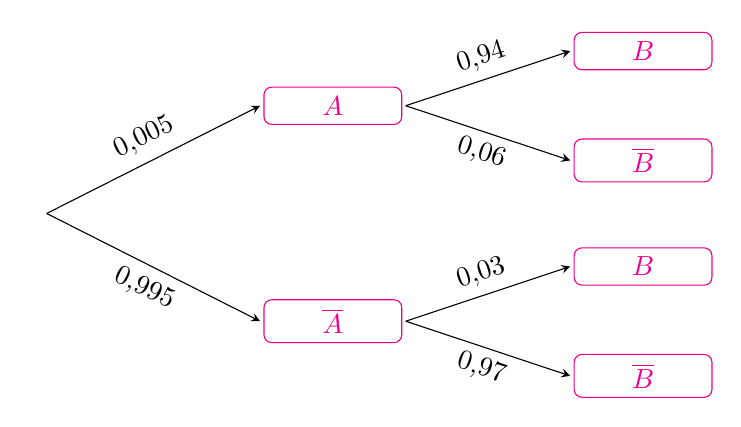
\begin{tikzpicture}
					\def\gocm{20} 
					 \def\gocn{10}
					\def\r{4} 
					 \tikzset{s/.style={outer sep=0.5 mm,draw,magenta,rectangle,minimum width=1.75cm,rounded corners=1mm}}
					\path (0,0) node (O){}++(\gocm:\r)  node[s](A1){$A$}++(\gocn:\r) node[s](A2){$B$};
					\path  (A1)++({-\gocn}:\r) node[s](a2){$\overline{B}$};
					\path  (O)++(-\gocm:\r) node[s](B1){$\overline{A}$}++(\gocn:\r) node[s](B2){$B$};
					\path (B1)++({-\gocn}:\r)  node[s](b2){$\overline{B}$};
					\foreach \x/\y  in {
						O/A1,A1/A2, 
						O/B1,B1/B2, 
						 A1/a2,
						 B1/b2}
					\draw[-stealth](\x.east)--(\y.west); 
					\path  (O)--(A1.west) node[pos=0.5,above,sloped]{$\mbox{0{,}005}$}
						(O)--(B1.west) node[pos=0.5,below,sloped]{$\mbox{0{,}995}$} 
						 (B1.east)--(B2.west) node[pos=0.5,above,sloped]{$\mbox{0{,}03}$}
						 (A1.east)--(A2.west) node[pos=0.5,above,sloped]{$\mbox{0{,}94}$}
						 (A1.east)--(a2.west) node[pos=0.5,below,sloped]{$\mbox{0{,}06}$}
						 (B1.east)--(b2.west) node[pos=0.5,below,sloped]{$\mbox{0{,}97}$};
				\end{tikzpicture}
		\end{center}
		Ta  thấy xác suất mắc bệnh hiểm nghèo Y của một người khi xét nghiệm cho kết quả dương tính là $\mathrm{P} \left(A|B\right)$. Áp dụng công thức Bayes, ta có
		$$\mathrm{P} \left(A|B\right)=\dfrac{\mathrm{P} \left(A\right) \cdot \mathrm{P}\left(B|A\right)}{\mathrm{P}\left(A\right) \cdot \mathrm{P}\left(B|A\right)+\mathrm{P} \left(\overline{A}\right) \cdot \mathrm{P} \left(B|\overline{A}\right)}=\dfrac{0{,}005 \cdot 0{,}94}{0{,}005 \cdot 0{,}94+0{,}995 \cdot  0{,}03}\approx 13{,}6\%.$$
		Vậy xác suất mắc bệnh hiểm nghèo Y của  một người khi xét nghiệm cho kết quả dương tính là $13{,}6\%$.
	 }
\end{bt}

% nguồn: Lop_12_Dai_so_Chuong_6
\begin{bt}%[2D6V2-4]%[ma:a51a427d]
	Tỉ lệ người dân đã tiêm vắc xin phòng bệnh A ở một địa phương là $65\%$. Trong số những người đã tiêm phòng, tỉ lệ mắc bệnh A là $5\%$; trong số những người chưa tiêm, tỉ lệ mắc bệnh A là $17\%$. Chọn ngẫu nhiên một người ở địa phương đó. Biết rằng người đó mắc bệnh A. Tính xác suất người đó không tiêm vắc xin  phòng bệnh A.
	 \loigiai{
		Gọi $X$ là biến cố \lq\lq Người  dân được tiêm phòng bệnh A\rq\rq. \\
		$Y$ là biến cố \lq\lq  Người dân mắc bệnh A\rq\rq . \\
		 Ta có
		$\mathrm{P} \left(X\right)=0{,}65$; $\mathrm{P} \left(\overline{X}\right)=0{,}35$.\\ 
		Tỉ lệ mắc bệnh  khi tiêm phòng là $\mathrm{P} \left(Y|X\right)=0{,}05$.\\
		Tỉ lệ mắc bệnh khi chưa tiêm phòng là $\mathrm{P}  \left(Y|\overline{X}\right)=0{,}17$.\\
		 Xác suất người này mắc bệnh $A$ là
		\[\mathrm{P} \left(Y\right)=\mathrm{P} \left(X\right) \cdot \mathrm{P} \left(Y|X\right)+\mathrm{P} \left(\overline{X}\right) \cdot \mathrm{P} \left(Y|\overline{X}\right)=0{,}65 \cdot 0{,}05+0{,}35  \cdot 0{,}17=0{,}092.\]
		Xác suất để  người bệnh không tiêm phòng là\\
		\[\mathrm{P} \left(\overline{X}|Y\right)=\dfrac{\mathrm{P} \left(\overline{X}\right) \cdot \mathrm{P} \left(Y|\overline{X}\right)}{\mathrm{P}\left(Y\right)}=\dfrac{0{,}35  \cdot 0{,}17}{0{,}092}=\dfrac{119}{184}.\]
	 }
\end{bt}

% nguồn: Lop_12_Dai_so_Chuong_6
\begin{bt}%[2D6V2-4]%[ma:7e197b89]
	Trong một trường học, tỉ lệ học sinh nữ là $52\%$. Tỉ lệ học sinh nữ và tỉ  lệ học sinh nam tham gia câu lạc bộ nghệ thuật lần lượt là $18\%$ và $15\%$. Chọn ngẫu nhiên một học sinh của trường. Biết rằng học sinh được chọn có tham gia câu lạc bộ nghệ thuật. Tính xác suất học sinh đó là nam.
	 \loigiai{
		Gọi $A$ là biến cố  \lq\lq Học sinh được chọn là học sinh nữ \rq\rq~ và $B$ là biến cố \lq\lq Học sinh được chọn tham gia câu lạc bộ nghệ thuật\rq\rq .\\
		Khi đó ta có  $\mathrm{P} \left(A\right)=0{,}52$; $\mathrm{P} \left(\overline{A}\right)=1-\mathrm{P}\left(A \right)=0{,}48$; $\mathrm{P}\left(B|A\right)=0{,}18$; $\mathrm{P}\left(B|\overline{A}\right)=0{,}15$.\\
		Áp dụng công thức xác  suất toàn phần ta có
		\[\mathrm{P}  \left(B\right)=\mathrm{P} \left(A\right)\mathrm{P} \left(B|A\right)+\mathrm{P} \left(\overline{A}\right)\mathrm{P} \left(B|\overline{A}\right)=0{,}52 \cdot 0{,}18+0{,}48 \cdot 0{,}15=0{,}1656.\]
		Xác suất học sinh đó là nam bằng 
		\[\mathrm{P} \left(\overline{A}|B\right)=\dfrac{\mathrm{P} \left(\overline{A}\right)  \cdot \mathrm{P} \left(B|\overline{A}\right)}{\mathrm{P}\left(B\right)}=\dfrac{0{,}48 \cdot 0{,}15}{0{,}1656}=\dfrac{10}{23}.\]
	} 
\end{bt}
